\section{Measuring market power: markups, margins and concentration}\label{sec:02-measures}

Every question in this chapter concerns the gap between price and marginal cost. \Cref{sec:01-lerner} and
\cref{sec:01-concentration} defined the measures of that gap, and the measures of market structure, that the rest
of the book uses. This section recalls them in the notation of this chapter and adds the algebra that later
sections need.

\subsection{Market power and margins}\label{sec:02-margins}

We use the definitions of \cref{def:01-market-power}. A firm has market power if it can profitably set a price
above its marginal cost. The benchmark is the price-taking firm, which treats the price $p$ as given and chooses
its output $q$ to maximize $pq - C(q)$. At an interior optimum it produces where $p = C'(q)$, so the gap we wish to
measure is zero. In this chapter $c$ denotes a constant marginal cost. When marginal cost varies with output, every
measure below applies with $c$ replaced by $C'(q)$.

With price $p$ and marginal cost $c > 0$, the four measures of \cref{def:01-market-power} are the dollar markup
$p - c$, the Lerner index $L = \frac{p - c}{p}$, the markup ratio $\mu = \frac{p}{c}$ and the markup rate
$\mu - 1 = \frac{p - c}{c}$. The Lerner index and the markup ratio carry the same information, as
\eqref{eq:01-lerner-mu} shows:
\begin{align*}
  L = \frac{p - c}{p} &= 1 - \frac{c}{p} = 1 - \frac{1}{\mu} = \frac{\mu - 1}{\mu}, \\
  \frac{1}{\mu} &= 1 - L, \qquad\text{so}\qquad \mu = \frac{1}{1 - L} .
\end{align*}
When $0 < c \le p$, the Lerner index lies in $[0, 1)$ and $\mu \ge 1$. A price 25 percent above marginal cost has
$\mu = 1.25$ and $L = \frac{0.25}{1.25} = 0.20$. Market power is a statement about the margin on the last unit sold.
It says nothing directly about profit, which also depends on fixed costs. The dollar markup is measured in
currency, while $L$ and $\mu$ are pure numbers. The dollar markup is the natural object in the pricing first-order
condition (\cref{sec:02-monopoly}). The Lerner index is the natural object when we compare industries, because it
does not depend on units.

\begin{remark}[Positive margins are not evidence of rents]\label{rem:02-fixed-costs}
Consider a firm with constant marginal cost $c$ and fixed cost $F$ that sells $q$ units at price $p$. Its profit is
$\pi = (p - c)q - F$. Dividing by revenue $pq$ gives
\[
  \frac{\pi}{pq} = \frac{p - c}{p} - \frac{F}{pq} = L - \frac{F}{pq} .
\]
The profit margin on sales equals the Lerner index minus the share of revenue absorbed by fixed costs. Under free
entry profit is driven to zero, and then
\[
  p = c + \frac{F}{q}, \qquad L = \frac{F}{pq} > 0 .
\]
A firm that earns no economic rent therefore has a strictly positive Lerner index whenever it has fixed costs.
Such a firm needs a positive margin to survive. Evidence of high markups must be weighed against fixed and sunk
costs before it can be read as evidence of excess profit. The same point runs through the recent debate on rising
markups \citep{DeLoeckerEeckhoutUnger2020}, which \cref{ch:intro} reviews. \Cref{sec:02-entry} shows that free
entry ties the Cournot markup exactly to the fixed cost.
\end{remark}

Measured margins raise a further problem. Accounting data report average rather than marginal cost, allocate common
costs by convention, and use accounting depreciation. Margins computed from them are not $\frac{p - c}{p}$, as
\cref{ch:intro} explains. For this reason the methods in this book usually infer marginal cost from behavior
(\cref{sec:02-infer-mc}).

\subsection{Concentration}\label{sec:02-concentration}

Market structure is summarized by the concentration measures of \cref{def:01-concentration}. Consider $N$ firms
that sell a homogeneous good, with outputs $q_i$, industry output $Q = \sum_{i=1}^N q_i$ and market shares
$s_i = \frac{q_i}{Q}$. We write $s_{(1)} \ge s_{(2)} \ge \dots \ge s_{(N)}$ for the shares in decreasing order. The
$m$-firm concentration ratio is $\mathit{CR}_m = \sum_{i=1}^{m} s_{(i)}$, and the Herfindahl-Hirschman index is
$\HHI = \sum_{i=1}^N s_i^2$, quoted in HHI points as $10{,}000 \times \HHI$. Its numbers equivalent
$\frac{1}{\HHI}$ is the number of equal-sized firms that would produce the same index. \Cref{ch:intro} writes it
as $N^{\mathrm{eq}}$. In this chapter $N^e$ denotes a different object, the free-entry number of firms
(\cref{sec:02-entry}).

By \cref{prop:01-hhi-variance}, the index decomposes as
\[
  \HHI = \frac{1}{N} + N\sigma_s^2, \qquad \sigma_s^2 = \frac{1}{N}\sum_{i=1}^N \left(s_i - \frac{1}{N}\right)^2,
\]
where $\sigma_s^2$ is the cross-firm variance of shares around their mean $\frac{1}{N}$. Hence
$\frac{1}{N} \le \HHI \le 1$. The term $\frac{1}{N}$ reflects the number of firms, and the term $N\sigma_s^2$
reflects the inequality of their sizes. \Cref{cor:02-efficient} uses the decomposition to show that cost
differences raise concentration in a Cournot market with general demand.

The index also has a simple rule for mergers. Suppose firms $i$ and $j$ combine and every share stays at its
premerger value. The merged firm then has share $s_i + s_j$, and the index changes by
\begin{equation}\label{eq:02-delta-hhi}
  \Delta\HHI = (s_i + s_j)^2 - s_i^2 - s_j^2 = 2s_is_j .
\end{equation}
A merger of firms with 20 and 10 percent of the market raises the index by $2 \times 0.2 \times 0.1 = 0.04$, or
400 HHI points. Merger guidelines use this formula as a screen (\cref{ch:mergers}). It holds shares fixed, which no
equilibrium model implies. \Cref{rem:02-cournot-merger} shows that in symmetric Cournot competition the formula
overstates the change in concentration whenever more than two firms are present.

The Herfindahl index belongs to a wider family. \citet{EncaouaJacquemin1980} ask which indices deserve to be called
measures of concentration \citep[sec.~5.5]{Tirole1988}. They require three properties of an index
$R(s_1, \dots, s_N)$: symmetry in the shares, the Lorenz condition, and no rise with the number of equal-sized
firms. \Cref{rem:01-ej-axioms} states these properties and shows that every index of the form
\begin{equation}\label{eq:02-ej-family}
  R(s_1, \dots, s_N) = \sum_{i=1}^N s_i\, h(s_i),
\end{equation}
with $h$ nondecreasing and $s\, h(s)$ convex, satisfies them. The symbols $R$ and $h$ are local to this subsection.
The Herfindahl index has $h(s) = s$, and the entropy index $\sum_i s_i\ln s_i$ has $h(s) = \ln s$. The ratio
$\mathit{CR}_m$ satisfies the three properties, but it is not of the form \eqref{eq:02-ej-family}. It satisfies the
Lorenz condition only weakly, since a small transfer between two of the $m$ largest firms leaves $\mathit{CR}_m$
unchanged. The properties rank distributions of shares, but they do not say what an index measures. The Cournot
model links the Herfindahl index to margins and profits (\cref{sec:02-cournot-markups}), and Stigler's model links
it to the detection of secret price cuts (\cref{sec:02-stigler}).

Every concentration index presupposes a market. The analyst must choose the set of products and the geographic
area within which shares are computed. With differentiated products this choice is often contestable, and
\cref{ch:diffprod,ch:mergers} discuss how demand estimates can discipline it.

\section{Monopoly pricing}\label{sec:02-monopoly}

A single seller facing a downward-sloping demand curve is the simplest setting with market power. Its pricing rule
reappears in every later model, because each firm in an oligopoly behaves as a monopolist on its own residual
demand. This section derives the rule and states the conditions under which it characterizes the optimum. It then
shows how the rule can be inverted to recover marginal cost and works through the demand curves that recur in
applied work.

\subsection{The pricing problem}\label{sec:02-monopoly-foc}

\begin{assumption}[Monopoly]\label{ass:02-monopoly}
A single firm faces market demand $Q(p)$, which is twice continuously differentiable with $Q(p) > 0$ and
$Q'(p) < 0$ on the relevant range of prices. Marginal cost is a constant $c \ge 0$. The firm chooses $p$ to maximize
profit $\pi(p) = (p - c)Q(p)$.
\end{assumption}

Differentiating profit gives the first-order condition
\begin{equation}\label{eq:02-foc-monopoly}
  \pi'(p) = Q'(p)(p - c) + Q(p) = 0 .
\end{equation}
A small price increase has two effects. It raises revenue on the $Q(p)$ units still sold, and it loses the margin
$p - c$ on the $-Q'(p)$ units that customers no longer buy. At the optimum the two effects balance. The
second-order condition for a local maximum is
\begin{equation}\label{eq:02-soc-monopoly}
  \pi''(p) = Q''(p)(p - c) + 2Q'(p) < 0 .
\end{equation}

\begin{lemma}[Second-order condition and uniqueness]\label{lem:02-soc}
Let \cref{ass:02-monopoly} hold.
\begin{enumerate}[label=(\roman*)]
  \item At any price satisfying \eqref{eq:02-foc-monopoly}, the second-order condition \eqref{eq:02-soc-monopoly}
  holds if and only if $Q(p)Q''(p) < 2Q'(p)^2$.
  \item The inequality in (i) holds whenever $\ln Q$ is concave at $p$.
  \item If $\ln Q$ is concave on the whole range of prices, at most one price satisfies
  \eqref{eq:02-foc-monopoly}, and such a price maximizes profit.
\end{enumerate}
\end{lemma}

\begin{proof}
For (i), the first-order condition gives $p - c = -\frac{Q(p)}{Q'(p)}$. Substituting into $\pi''(p)$,
\begin{align*}
  \pi''(p) &= -\frac{Q(p)Q''(p)}{Q'(p)} + 2Q'(p) \\
           &= \frac{2Q'(p)^2 - Q(p)Q''(p)}{Q'(p)} .
\end{align*}
The denominator is negative, so $\pi''(p) < 0$ if and only if the numerator is positive. For (ii), the second
derivative of $\ln Q$ is
\[
  \frac{\dd^2 \ln Q(p)}{\dd p^2} = \frac{Q(p)Q''(p) - Q'(p)^2}{Q(p)^2} .
\]
Concavity makes it nonpositive, so $QQ'' \le (Q')^2 < 2(Q')^2$. For (iii), define $m(p) = -\frac{Q(p)}{Q'(p)} > 0$
and factor the derivative of profit as
\[
  \pi'(p) = Q'(p)\left[(p - c) - m(p)\right] .
\]
Since $\frac{1}{m(p)} = -\frac{\dd \ln Q(p)}{\dd p}$, concavity of $\ln Q$ makes $\frac{1}{m}$ nondecreasing and
hence $m$ nonincreasing. The bracket $h(p) = p - c - m(p)$ is then strictly increasing, so it has at most one zero.
Because $Q' < 0$, profit rises where $h < 0$ and falls where $h > 0$. A zero of $h$ is therefore a global maximum.
\end{proof}

A function whose logarithm is concave is called \emph{log-concave}. Linear and exponential demand curves are
log-concave. So is any demand curve $Q(p) = M[1 - G(p)]$ generated by a distribution $G$ of willingness to pay with
a log-concave density (\cref{app:math}). Constant-elasticity demand is log-convex, so \cref{lem:02-soc}(ii) does not
cover it, and \cref{ex:02-ce} checks the conditions directly.

\citet[sec.~1.1.1.4]{Tirole1988} locates the difficulty in revenue. Revenue $R(p) = pQ(p)$ has second derivative
$R''(p) = 2Q'(p) + pQ''(p)$. The first term is negative, and the second is nonpositive when demand is concave. With
constant marginal cost, $\pi''(p) = 2Q'(p) + (p - c)Q''(p)$ is then negative at every $p \ge c$, so concave demand
makes profit concave on the relevant range. Convex demand can make revenue, and with it profit, fail to be concave,
which is why \cref{lem:02-soc} works with the weaker property of log-concavity.

The first-order condition can be arranged in two ways, and the book uses both throughout. \Cref{prop:01-pricing-rule}
stated both for residual demand. We repeat the two short steps because later sections build on each. For the first
arrangement, divide \eqref{eq:02-foc-monopoly} by $-Q'(p) > 0$ and solve for the margin:
\begin{align*}
  -(p - c) - \frac{Q(p)}{Q'(p)} &= 0, \\
  p - c &= -\frac{Q(p)}{Q'(p)} .
\end{align*}
We call the right side the dollar markup $m(p)$ and record
\begin{equation}\label{eq:02-dollar-markup}
  p - c = m(p) \equiv -\frac{Q(p)}{Q'(p)} = \frac{1}{-\frac{\dd \ln Q(p)}{\dd p}} .
\end{equation}
The quantity $-\frac{\dd \ln Q}{\dd p} = -\frac{Q'(p)}{Q(p)}$ is the \emph{semi-elasticity} of demand, the
proportional fall in quantity per dollar of price increase. The dollar markup is its reciprocal. If a one-dollar
price increase loses 5 percent of sales, the markup is 20 dollars. Equation \eqref{eq:02-dollar-markup} involves
only the demand curve, evaluated at the optimal price. Marginal cost affects the markup only through the choice of
that price.

For the second arrangement, divide \eqref{eq:02-dollar-markup} by $p$:
\begin{equation}\label{eq:02-lerner}
  \frac{p - c}{p} = -\frac{Q(p)}{p\,Q'(p)} = \frac{1}{\varepsilon(p)}, \qquad
  \varepsilon(p) = -Q'(p)\frac{p}{Q(p)} > 0 .
\end{equation}
This is the \emph{Lerner rule}, also called the \emph{inverse elasticity rule}. The Lerner index of a monopolist
equals the inverse of the price elasticity of demand at the chosen price. Multiplying by $p$ and collecting the
terms in $p$ expresses price as a multiple of cost:
\begin{align*}
  p - c &= \frac{p}{\varepsilon}, \\
  p\left(1 - \frac{1}{\varepsilon}\right) &= c,
\end{align*}
\begin{equation}\label{eq:02-ce-price}
  p = \frac{\varepsilon}{\varepsilon - 1}\,c .
\end{equation}
Both \eqref{eq:02-dollar-markup} and \eqref{eq:02-ce-price} are fixed-point conditions, because $m$ and
$\varepsilon$ generally depend on $p$. They become explicit pricing formulas only for special demand curves
(\cref{sec:02-demand-families}).

\begin{proposition}[A monopolist prices on the elastic part of demand]\label{prop:02-elastic}
Under \cref{ass:02-monopoly}, any price that satisfies \eqref{eq:02-foc-monopoly} has $p > c$ and
$\varepsilon(p) \ge 1$. If $c > 0$, then $\varepsilon(p) > 1$.
\end{proposition}

\begin{proof}
By \eqref{eq:02-dollar-markup}, $p - c = m(p) > 0$, because $Q > 0$ and $Q' < 0$. Hence $p > c \ge 0$, so the
Lerner index satisfies $0 < L \le 1$, with $L < 1$ when $c > 0$. By \eqref{eq:02-lerner}, $\frac{1}{\varepsilon} = L$.
Therefore $\varepsilon \ge 1$, and $\varepsilon > 1$ when $c > 0$.
\end{proof}

The intuition is direct. Where demand is inelastic, a small price increase raises revenue and reduces output, which
lowers cost. Both effects raise profit, so no such price can be optimal. With zero marginal cost the monopolist
maximizes revenue and sets $\varepsilon = 1$.

It is often convenient to let the firm choose output. Let $P(Q)$ be inverse demand. The firm chooses $Q$ to maximize
$P(Q)Q - cQ$, and the first-order condition equates marginal revenue to marginal cost:
\begin{equation}\label{eq:02-mr}
  MR(Q) = P(Q) + QP'(Q) = c .
\end{equation}
Factoring out the price gives
\[
  MR(Q) = P(Q)\left[1 + \frac{QP'(Q)}{P(Q)}\right] = P(Q)\left[1 - \frac{1}{\varepsilon}\right] .
\]
The second step uses $P'(Q) = \frac{1}{Q'(p)}$ at $p = P(Q)$, so that $\frac{QP'(Q)}{P(Q)} = \frac{Q}{pQ'(p)} =
-\frac{1}{\varepsilon}$. Setting $MR = c$ gives \eqref{eq:02-ce-price} again. The price and quantity formulations
are equivalent, and we move between them freely.

\begin{remark}[Rising marginal cost]\label{rem:02-convex-cost}
With a convex cost function $C(Q)$, profit is $pQ(p) - C(Q(p))$, and the first-order condition becomes
$Q'(p)\left[p - C'(Q(p))\right] + Q(p) = 0$. Every formula above holds with $c$ replaced by marginal cost at the
optimal output. The second derivative of profit becomes
\[
  \pi''(p) = Q''(p)\left[p - C'(Q)\right] + 2Q'(p) - C''(Q)\,Q'(p)^2 .
\]
The last term is nonpositive, so rising marginal cost makes the second-order condition easier to satisfy.
\end{remark}

One comparative static needs none of the conditions above. A higher marginal cost never lowers the monopoly price,
whatever the shapes of demand and cost. The proof compares two optima directly and is an example of a
\emph{revealed-preference argument}: each optimum must do at least as well as the other choice under its own cost.

\begin{lemma}[The monopoly price does not fall when marginal cost rises]\label{lem:02-monotone}
Let inverse demand $P(Q)$ be nonincreasing, and let $C_1$ and $C_2$ be differentiable cost functions with
$C_2'(q) > C_1'(q)$ for every $q > 0$. Let $q_k$ be an output that maximizes $P(q)q - C_k(q)$, and let
$p_k = P(q_k)$, for $k = 1, 2$. Then $q_1 \ge q_2$ and $p_1 \le p_2$.
\end{lemma}

\begin{proof}
Under $C_1$ the firm could have sold $q_2$ at the price $p_2$. Under $C_2$ it could have sold $q_1$ at $p_1$. So
\begin{align*}
  p_1q_1 - C_1(q_1) &\ge p_2q_2 - C_1(q_2), \\
  p_2q_2 - C_2(q_2) &\ge p_1q_1 - C_2(q_1) .
\end{align*}
Adding the two inequalities cancels the revenues and leaves
\[
  \bigl[C_2(q_1) - C_2(q_2)\bigr] - \bigl[C_1(q_1) - C_1(q_2)\bigr] \ge 0 ,
\]
which by the fundamental theorem of calculus reads
\[
  \int_{q_2}^{q_1}\bigl[C_2'(x) - C_1'(x)\bigr]\,\dd x \ge 0 .
\]
The integrand is positive. If $q_1 < q_2$ the integral would be negative, so $q_1 \ge q_2$. Since $P$ is
nonincreasing, $p_1 = P(q_1) \le P(q_2) = p_2$.
\end{proof}

The argument is that of \citet[sec.~1.1.1.1, eqs.~(1.2) to (1.5)]{Tirole1988}. It needs no second-order condition,
no differentiability of demand and no uniqueness of the optimum. With constant marginal costs $c_1 < c_2$ it says
that the monopoly price is nondecreasing in $c$. \Cref{prop:02-pt-monopoly} gives the rate of increase when demand
is smooth.

\subsection{Residual demand and the dominant firm}\label{sec:02-residual}

Nothing in the derivation of \eqref{eq:02-dollar-markup} and \eqref{eq:02-lerner} requires the firm to be alone in
its market. Any firm that sets its price against a given demand curve obeys the same rules. The \emph{residual
demand} of a firm is the quantity it sells at each of its own prices, given how its rivals behave. Its
\emph{residual elasticity} $\varepsilon^R$ is the elasticity of that curve. The \emph{market elasticity}
$\varepsilon$ is the elasticity of total industry demand. A firm with market power satisfies
$\frac{p - c}{p} = \frac{1}{\varepsilon^R}$, and the two elasticities coincide only for a monopolist.

The residual elasticity depends on how rivals respond. In a Cournot market (\cref{sec:02-cournot}), rivals hold
their total output $Q_{-i}$ fixed, so firm $i$ faces the residual inverse demand $P(q_i + Q_{-i})$. A change in
$q_i$ then changes industry output one for one, and
\begin{equation}\label{eq:02-cournot-residual}
  \varepsilon_i^R = -\frac{\dd q_i}{\dd p}\,\frac{p}{q_i}
    = -\frac{\dd Q}{\dd p}\,\frac{p}{Q}\cdot\frac{Q}{q_i} = \frac{\varepsilon}{s_i} .
\end{equation}
A firm with a small share faces very elastic residual demand even when market demand is inelastic. At the other
extreme, a firm whose rivals sell the same good at a fixed price faces infinitely elastic residual demand above that
price (\cref{sec:02-bertrand}). The next example derives the residual elasticity when rivals are price takers.

\begin{example}[Dominant firm with a competitive fringe]\label{ex:02-dominant}
A \emph{dominant firm} sets the price, and a \emph{competitive fringe} of small price-taking firms supplies $S(p)$
at each price, with $S'(p) \ge 0$. The dominant firm's residual demand is
\[
  Q_d(p) = Q(p) - S(p) .
\]
Let $s_d = \frac{Q_d}{Q}$ be the dominant firm's share and $\varepsilon_f = S'(p)\frac{p}{S(p)} \ge 0$ the
elasticity of fringe supply. Differentiating gives $Q_d'(p) = Q'(p) - S'(p)$, so
\begin{align*}
  \varepsilon^R = -Q_d'(p)\,\frac{p}{Q_d}
    &= -Q'(p)\,\frac{p}{Q}\cdot\frac{Q}{Q_d} + S'(p)\,\frac{p}{S}\cdot\frac{S}{Q_d} \\
    &= \frac{\varepsilon}{s_d} + \varepsilon_f\,\frac{1 - s_d}{s_d} .
\end{align*}
The second line uses $\frac{Q}{Q_d} = \frac{1}{s_d}$ and $\frac{S}{Q_d} = \frac{1 - s_d}{s_d}$. The Lerner rule then
gives the dominant firm's margin,
\begin{equation}\label{eq:02-dominant-lerner}
  L_d = \frac{1}{\varepsilon^R} = \frac{s_d}{\varepsilon + \varepsilon_f(1 - s_d)} .
\end{equation}
\citet{LandesPosner1981} proposed this formula as a guide to inferring market power from market shares in antitrust
cases. It shows that a large share alone does not imply a large margin. Take $s_d = 0.7$ and $\varepsilon = 2$. With
an unresponsive fringe ($\varepsilon_f = 0$), $L_d = \frac{0.7}{2} = 0.35$. With $\varepsilon_f = 10$, the residual
elasticity is $\frac{2}{0.7} + 10\cdot\frac{0.3}{0.7} \approx 7.14$ and $L_d = \frac{0.7}{2 + 3} = 0.14$. The
margin falls by 60 percent although the share is unchanged. What limits the dominant firm is the elasticity of the
demand it faces, and that elasticity depends on how quickly rivals expand.
\end{example}

The residual elasticity is the object that a firm's pricing reveals. \Cref{ch:conduct} shows how
\citet{BakerBresnahan1988} estimate the residual demand curve of a single firm directly.

\subsection{Multiproduct monopoly}\label{sec:02-multiproduct}

A firm that sells several products sets each price with an eye on the others. Let a monopolist sell products
$j = 1, \dots, J$ at prices $p = (p_1, \dots, p_J)$. Demand for product $j$ is $q_j(p)$, the cost of the output
vector is $C(q_1, \dots, q_J)$, and $mc_j = \frac{\partial C}{\partial q_j}$ is the marginal cost of product $j$. The
firm maximizes
\[
  \pi(p) = \sum_{k=1}^J p_k\, q_k(p) - C\bigl(q_1(p), \dots, q_J(p)\bigr) .
\]
Differentiating with respect to $p_j$ gives the first-order condition \citep[sec.~1.1.2, eq.~(1.6)]{Tirole1988}
\begin{equation}\label{eq:02-multi-foc}
  q_j + \sum_{k=1}^J p_k\frac{\partial q_k}{\partial p_j} = \sum_{k=1}^J mc_k\,\frac{\partial q_k}{\partial p_j},
  \qquad j = 1, \dots, J .
\end{equation}
The left side is the marginal revenue from raising $p_j$, including the revenue that the price change moves to the
firm's other products. The right side is the change in total cost. Collecting the terms product by product gives
\begin{equation}\label{eq:02-multi-foc-margin}
  q_j + (p_j - mc_j)\frac{\partial q_j}{\partial p_j} + \sum_{k \ne j}(p_k - mc_k)\frac{\partial q_k}{\partial p_j}
  = 0 .
\end{equation}
With independent demands, $\frac{\partial q_k}{\partial p_j} = 0$ for $k \ne j$, and each product obeys the
single-product rule \eqref{eq:02-lerner}. Products with less elastic demand then carry higher markups, the simplest
form of Ramsey pricing.

\casehead{The Lerner rule with cross effects} Let costs be separable, $C = \sum_k C_k(q_k)$, so that $mc_k$ depends on
$q_k$ alone. Write $\lvert\varepsilon_{jj}\rvert = -\frac{\partial q_j}{\partial p_j}\frac{p_j}{q_j}$ for the own-price
elasticity, $\varepsilon_{kj} = \frac{\partial q_k}{\partial p_j}\frac{p_j}{q_k}$ for the cross elasticity of
product $k$ with respect to the price of $j$, and $R_j = p_jq_j$ for the revenue of product $j$. Dividing
\eqref{eq:02-multi-foc-margin} by $q_j$ and substituting $\frac{\partial q_j}{\partial p_j} = -\lvert\varepsilon_{jj}
\rvert\frac{q_j}{p_j}$ and $\frac{\partial q_k}{\partial p_j} = \varepsilon_{kj}\frac{q_k}{p_j}$,
\[
  1 - \lvert\varepsilon_{jj}\rvert\,\frac{p_j - mc_j}{p_j} + \sum_{k \ne j}(p_k - mc_k)\,\frac{\varepsilon_{kj}\,q_k}
  {p_jq_j} = 0 .
\]
Solving for the Lerner index of product $j$ gives
\begin{equation}\label{eq:02-multi-lerner}
  \frac{p_j - mc_j}{p_j} = \frac{1}{\lvert\varepsilon_{jj}\rvert}
  + \sum_{k \ne j}\frac{(p_k - mc_k)\,q_k\,\varepsilon_{kj}}{R_j\,\lvert\varepsilon_{jj}\rvert} .
\end{equation}
This is Tirole's formula. He defines the cross elasticity with the opposite sign, so his version has a minus sign in
front of the sum. Suppose the other products earn positive margins. If they are \emph{substitutes} for product $j$
($\varepsilon_{kj} > 0$), the sum is positive and the Lerner index of $j$ exceeds $\frac{1}{\lvert\varepsilon_{jj}
\rvert}$. If they are \emph{complements} ($\varepsilon_{kj} < 0$), the Lerner index falls short of
$\frac{1}{\lvert\varepsilon_{jj}\rvert}$. It can even be negative, so that product $j$ is sold below marginal cost to
raise the demand for the others.

Tirole interprets the formula through the biases of a decentralized firm. Suppose the firm were run by $J$
independent divisions, each maximizing the profit $p_jq_j - C_j(q_j)$ of its own product. Each division would set
the single-product markup $\frac{1}{\lvert\varepsilon_{jj}\rvert}$. With substitutes, a higher $p_j$ raises the sales
of the other divisions, and division $j$ ignores the margins it creates for them. The divisions are then de facto
competitors, and each prices too low from the point of view of the firm. With complements, each division prices too
high. Joint pricing internalizes these externalities between divisions. \Cref{sec:02-bridge} shows that the same
first-order condition, written with diversion ratios, governs multiproduct firms in oligopoly.

\begin{example}[Perfect complements]\label{ex:02-complements}
A firm sells nuts (product 1) and bolts (product 2), which are used one for one, so demand depends only on the total
price: $q_1 = q_2 = D(p_1 + p_2)$ \citep[Exercise~1.5]{Tirole1988}. Then $\frac{\partial q_k}{\partial p_j} =
D'(p_1 + p_2)$ for both $j$ and $k$. Writing $\bar P = p_1 + p_2$, condition \eqref{eq:02-multi-foc-margin} for
either product reads
\[
  D(\bar P) + (\bar P - mc_1 - mc_2)\,D'(\bar P) = 0 .
\]
This is the monopoly condition \eqref{eq:02-foc-monopoly} for a single composite good with price $\bar P$ and marginal
cost $mc_1 + mc_2$. Only the total price is determined. Compare two separate monopolists, one for each product. Each
sets $D(\bar P) + (p_j - mc_j)D'(\bar P) = 0$, so $p_j - mc_j = m(\bar P)$, with $m$ the dollar markup of
\eqref{eq:02-dollar-markup}. Adding the two conditions gives $\bar P - mc_1 - mc_2 = 2m(\bar P)$, twice the markup
$m(\bar P)$ that the integrated firm charges at its own price. When $m$ is nonincreasing, as under log-concave demand,
separate pricing therefore leads to a higher total price.
\end{example}

\casehead{Intertemporal applications} The same logic applies to one good sold at two dates, since the good at each
date is a separate product \citep[sec.~1.1.2]{Tirole1988}. Let $\delta \in (0, 1)$ be the firm's discount factor, as
in \cref{sec:02-repeated} and \cref{ch:collusion-theory}. The symbol differs from the mean utility $\delta_j$ of the
logit demand in \cref{ex:02-pt-examples} and later chapters. With \emph{goodwill}, a lower first-period price
raises second-period demand. Demand is $q_1 = D_1(p_1)$ in period 1 and $q_2 = D_2(p_2, p_1)$ in period 2,
with $\frac{\partial D_2}{\partial p_1} < 0$.
First-period demand does not depend on $p_2$, so the firm charges the monopoly price of
\eqref{eq:02-lerner} in period 2, given the goodwill it has built. In period 1 it charges less than the static
monopoly price. To see this, let $S(p_1) = p_1D_1(p_1) - C_1(D_1(p_1))$ be first-period profit and $V(p_1)$ the
maximized second-period profit. By the envelope theorem (\cref{app:math}),
\[
  V'(p_1) = (p_2 - mc_2)\,\frac{\partial D_2}{\partial p_1} < 0 ,
\]
since the second-period margin is positive. Let $p^s$ maximize $S$ and $p^*$ maximize $S + \delta V$. Optimality
gives $S(p^s) \ge S(p^*)$ and $S(p^*) + \delta V(p^*) \ge S(p^s) + \delta V(p^s)$. Adding the two inequalities gives
$V(p^*) \ge V(p^s)$, and since $V$ is decreasing, $p^* \le p^s$. The inequality is strict at an interior optimum.
There $S'(p^s) = 0$ and $\delta V'(p^s) < 0$. A small price cut from $p^s$ therefore raises $S + \delta V$. The
firm sacrifices current profit to raise future demand.

With \emph{learning by doing}, first-period output lowers second-period cost. Let the second-period cost be
$C_2(q_2, q_1)$ with $\frac{\partial C_2}{\partial q_1} < 0$, and let $V(q_1)$ be the maximized second-period profit.
The firm chooses $q_1$ to maximize $P_1(q_1)q_1 - \tilde C(q_1)$, with the effective cost $\tilde C(q_1) = C_1(q_1) -
\delta V(q_1)$. By the envelope theorem, its marginal cost is
\[
  \tilde C'(q_1) = C_1'(q_1) + \delta\,\frac{\partial C_2}{\partial q_1} < C_1'(q_1) .
\]
First-period marginal revenue therefore falls short of current marginal cost. By \cref{lem:02-monotone}, which
compares two cost functions for the same demand, the first-period price lies weakly below the myopic monopoly price.
Tirole adds that with stationary demand and costs that fall with experience, output grows over time.

\subsection{Inferring marginal cost from prices}\label{sec:02-infer-mc}

The pricing rule can be read backward. If demand is known and the firm behaves as a monopolist, the first-order
condition determines marginal cost from the observed price and quantity:
\begin{equation}\label{eq:02-infer-mc}
  \hat c = p + \frac{Q(p)}{\hat Q'(p)} = p\left(1 - \frac{1}{\hat\varepsilon}\right) .
\end{equation}
Here $\hat Q'(p)$ and $\hat\varepsilon$ are estimates of the demand slope and elasticity at the observed price. The
first form follows from \eqref{eq:02-dollar-markup} and the second from \eqref{eq:02-lerner}. No cost data are
needed. This inversion is the core of the \emph{New Empirical Industrial Organization} (NEIO), the approach based on
studies of single industries that \citet{Bresnahan1989} surveys. Bresnahan lists as its first premise that
price-cost margins are not observable, so that the analyst infers marginal cost from firm behavior (p.~1012). He
quotes the title of \citet{Rosse1970}, ``Estimating Cost Function Parameters without Using Cost Data,'' as a
statement of the program (p.~1014).

Bresnahan's stylized model makes the inversion econometric. Observation $t$ has inverse market demand
$P(Q_t, Y_t, \epsilon_{dt})$, with demand shifters $Y_t$ and a demand error $\epsilon_{dt}$. Firm $i$ has marginal
cost $MC(q_{it}, W_{it}, Z_{it}, \epsilon_{cit})$, with factor prices $W_{it}$, other cost shifters $Z_{it}$ and a
cost error $\epsilon_{cit}$. Both functions are known up to unknown parameters. In our notation, his supply relation
(eq.~(4), p.~1016) is
\begin{equation}\label{eq:02-bresnahan-supply}
  P_t = MC(q_{it}, W_{it}, Z_{it}, \epsilon_{cit})
        - \theta_{it}\, q_{it}\, \frac{\partial P(Q_t, Y_t, \epsilon_{dt})}{\partial Q} .
\end{equation}
With a single firm and $\theta_{it} = 1$, the second term is $-QP'(Q)$, and \eqref{eq:02-bresnahan-supply} says
that marginal revenue equals marginal cost. With $\theta_{it} = 0$ it is the competitive supply curve $P = MC$.
Bresnahan stresses that marginal cost enters as a function of unknown parameters, never as an accounting datum.
Demand, cost and conduct parameters are estimated together. \Cref{sec:02-conduct} develops the conduct parameter
$\theta$, and \cref{ch:conduct} studies how data identify it. With conduct $\theta$ the inversion becomes
$\hat c = p + \theta\frac{Q}{\hat Q'(p)}$.

Two features of \eqref{eq:02-infer-mc} matter in practice. The first is that the implied cost inherits the sampling
error of the demand estimate, most strongly when demand is close to unit elastic. Differentiating
\eqref{eq:02-infer-mc} with respect to the elasticity gives $\frac{\partial \hat c}{\partial \hat\varepsilon} =
\frac{p}{\hat\varepsilon^2}$. By the delta method (\cref{app:econometrics}),
\[
  \operatorname{se}(\hat c) \approx \frac{p}{\hat\varepsilon^2}\,\operatorname{se}(\hat\varepsilon) .
\]
Take $p = 10$ and $\operatorname{se}(\hat\varepsilon) = 0.25$. At $\hat\varepsilon = 2$ the implied cost is 5, with
a standard error of about 0.63. At $\hat\varepsilon = 1.25$ it is 2, with a standard error of 1.6. An estimated
elasticity below one implies a negative marginal cost, which is inconsistent with monopoly pricing
(\cref{prop:02-elastic}). \Cref{ch:conduct} returns to this point for industries with inelastic demand, such as
electricity.

The second feature is that the inverted costs can be related to observed cost shifters. Suppose marginal cost is
$mc_t = w_t\psi + \omega_t$, with a row vector of cost shifters $w_t$, coefficients $\psi$ and an unobserved cost
shock $\omega_t$. Substituting \eqref{eq:02-infer-mc} gives the regression
\begin{equation}\label{eq:02-mc-regression}
  p_t + \frac{Q_t}{\hat Q'(p_t)} = w_t\psi + \omega_t .
\end{equation}
The left side is computed from data and estimated demand. If marginal cost also rises with output, $Q_t$ enters the
right side. Output is correlated with the cost shock $\omega_t$, so it must be instrumented, typically with demand
shifters. The additive cost shock is what makes the estimating equation linear in $\psi$. \Cref{ch:diffprod}
extends the inversion to firms that sell several differentiated products, where the markup involves the full matrix
of demand derivatives.

\subsection{Worked demand families}\label{sec:02-demand-families}

Four families of demand curves recur in applied work. Each gives an explicit monopoly price, and each implies a
different relation between cost and price. \Cref{fig:02-monopoly} illustrates the linear case.

\begin{example}[Linear demand]\label{ex:02-linear-monopoly}
Let $P(Q) = a - bQ$ with $a > c \ge 0$ and $b > 0$, so that $Q(p) = \frac{a - p}{b}$. Marginal revenue is
$a - 2bQ$. Setting it equal to $c$ and solving,
\begin{align*}
  a - 2bQ &= c, \\
  Q^m &= \frac{a - c}{2b}, \\
  p^m = a - bQ^m &= a - \frac{a - c}{2} = \frac{a + c}{2} .
\end{align*}
Since $Q'(p) = -\frac{1}{b}$, the elasticity at price $p$ is $\varepsilon(p) = \frac{1}{b}\cdot\frac{p}{Q(p)} =
\frac{p}{a - p}$. At the monopoly price,
\[
  \varepsilon(p^m) = \frac{\frac{a + c}{2}}{\frac{a - c}{2}} = \frac{a + c}{a - c}, \qquad
  L = \frac{p^m - c}{p^m} = \frac{a - c}{a + c} = \frac{1}{\varepsilon(p^m)} .
\]
The dollar markup is $m(p) = -\frac{Q(p)}{Q'(p)} = a - p$, which falls one for one with price. At the optimum it
equals $\frac{a - c}{2}$, so each dollar of marginal cost raises the monopoly price by fifty cents. With $a = 10$,
$b = 1$ and $c = 2$, we obtain $Q^m = 4$, $p^m = 6$, $\varepsilon(p^m) = \frac{3}{2}$ and $L = \frac{2}{3}$.
\end{example}

\begin{figure}[htbp]
\centering
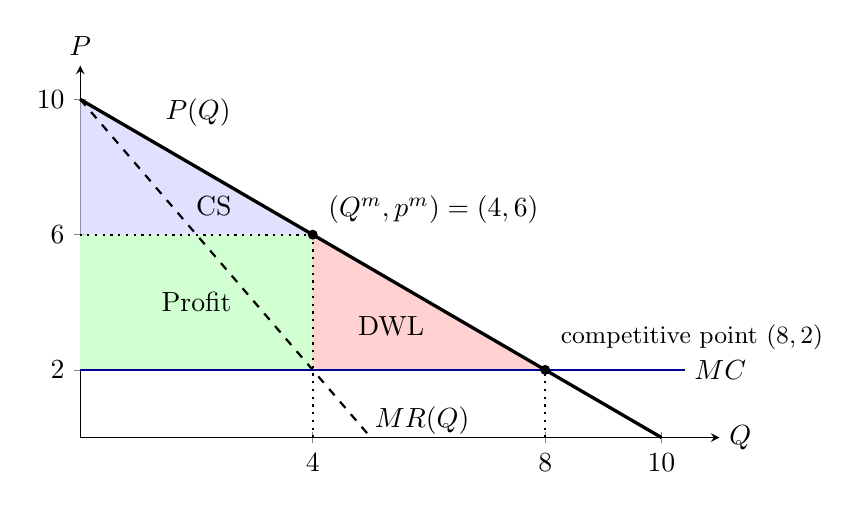
\begin{tikzpicture}
\begin{axis}[
  width=0.80\textwidth, height=0.52\textwidth,
  axis lines=left,
  xmin=0, xmax=11, ymin=0, ymax=11,
  xlabel={$Q$}, ylabel={$P$},
  xtick={4,8,10}, ytick={2,6,10},
  every axis x label/.style={at={(current axis.right of origin)}, anchor=west},
  every axis y label/.style={at={(current axis.above origin)}, anchor=south},
  clip=false]
  \fill[blue!12] (axis cs:0,6) -- (axis cs:0,10) -- (axis cs:4,6) -- cycle;
  \fill[green!18] (axis cs:0,2) rectangle (axis cs:4,6);
  \fill[red!18] (axis cs:4,6) -- (axis cs:4,2) -- (axis cs:8,2) -- cycle;
  \addplot[very thick, black, domain=0:10] {10 - x};
  \addplot[thick, dashed, black, domain=0:5] {10 - 2*x};
  \addplot[thick, blue!60!black, domain=0:10.4] {2};
  \draw[dotted, thick] (axis cs:4,0) -- (axis cs:4,6) -- (axis cs:0,6);
  \draw[dotted, thick] (axis cs:8,0) -- (axis cs:8,2);
  \fill (axis cs:4,6) circle (1.8pt);
  \fill (axis cs:8,2) circle (1.8pt);
  \node[anchor=south west] at (axis cs:4.1,6.05) {$(Q^m, p^m) = (4, 6)$};
  \node[anchor=south west, font=\small] at (axis cs:8.1,2.3) {competitive point $(8, 2)$};
  \node[anchor=south west] at (axis cs:1.3,8.9) {$P(Q)$};
  \node[anchor=west] at (axis cs:4.9,0.5) {$MR(Q)$};
  \node[anchor=west] at (axis cs:10.4,2) {$MC$};
  \node at (axis cs:2.3,6.85) {CS};
  \node at (axis cs:2,4) {Profit};
  \node at (axis cs:5.35,3.3) {DWL};
\end{axis}
\end{tikzpicture}
\caption{Monopoly with linear demand $P(Q) = 10 - Q$, marginal revenue $MR(Q) = 10 - 2Q$ and constant marginal cost
$MC = 2$. The monopolist sells $Q^m = 4$ at $p^m = 6$, while price taking would give the point $(8, 2)$. The
shaded areas are consumer surplus (CS), profit, and the deadweight loss (DWL) of pricing above marginal cost.
\Cref{sec:02-surplus} defines these areas formally. The Lerner index is $L = \frac{6 - 2}{6} = \frac{2}{3}$, which equals $\frac{1}{\varepsilon(p^m)} = \frac{2}{3}$ because
$\varepsilon(p^m) = \frac{6}{4} = \frac{3}{2}$.}
\label{fig:02-monopoly}
\end{figure}

\begin{example}[Constant-elasticity demand]\label{ex:02-ce}
Let $Q(p) = Ap^{-\varepsilon}$ with $A > 0$ and a constant $\varepsilon > 0$, and let marginal cost be strictly
positive, $c > 0$. The elasticity is the same at every price:
\[
  -Q'(p)\,\frac{p}{Q(p)} = \varepsilon A p^{-\varepsilon - 1}\cdot\frac{p}{Ap^{-\varepsilon}} = \varepsilon .
\]
If $\varepsilon > 1$, \eqref{eq:02-ce-price} is an explicit pricing formula, $p^m = \frac{\varepsilon}{\varepsilon -
1}c$. The Lerner index is the constant $\frac{1}{\varepsilon}$, and price is proportional to cost. The dollar markup
$m(p) = \frac{p}{\varepsilon}$ rises with price, so a one-dollar increase in cost raises price by
$\frac{\varepsilon}{\varepsilon - 1} > 1$ dollars. This demand curve is log-convex, so we check optimality
directly. Here $\frac{QQ''}{(Q')^2} = \frac{\varepsilon + 1}{\varepsilon}$, which is below 2 exactly when
$\varepsilon > 1$. The function $h(p) = p - c - \frac{p}{\varepsilon} = p\left(1 - \frac{1}{\varepsilon}\right) -
c$ is then strictly increasing, so the argument of \cref{lem:02-soc}(iii) shows that $p^m$ is the unique optimum. If
$\varepsilon \le 1$, revenue $Ap^{1 - \varepsilon}$ does not fall as price rises while cost $cAp^{-\varepsilon}$
falls, so profit rises at every price and no optimal price exists. \citet[Exercise~1.4]{Tirole1988} extends the
result to any convex cost function. With constant-elasticity demand and $\varepsilon > 1$, profit is then
quasi-concave in price. The boundary case $c = 0$, which \cref{ass:02-monopoly} allows, behaves differently
because profit equals revenue $Ap^{1 - \varepsilon}$. For $\varepsilon > 1$ profit rises without bound as price
falls toward zero, and the formula's value $p^m = 0$ is not an admissible price, so no optimum exists. For
$\varepsilon = 1$ profit equals $A$ at every price, so every positive price is optimal. For $\varepsilon < 1$
profit rises without bound in price.
\end{example}

\begin{example}[Exponential demand]\label{ex:02-exponential}
Let $Q(p) = e^{\frac{a - p}{b}}$ with $b > 0$, or equivalently $P(Q) = a - b\ln Q$. Then $Q'(p) = -\frac{1}{b}Q(p)$,
so the semi-elasticity is the constant $\frac{1}{b}$ and the dollar markup is $m(p) = -\frac{Q(p)}{Q'(p)} = b$ at
every price. The monopoly price is
\[
  p^m = c + b .
\]
A monopolist facing this demand charges a fixed dollar margin whatever its cost, so each dollar of cost passes
fully into price, exactly as under perfect competition. The elasticity $\varepsilon(p) = \frac{p}{b}$ rises with
price. Since $\ln Q = \frac{a - p}{b}$ is linear, and hence weakly concave, \cref{lem:02-soc} applies.
\end{example}

\begin{example}[The Bulow-Pfleiderer family]\label{ex:02-bp}
Consider demand curves of the form
\begin{equation}\label{eq:02-bp-demand}
  Q(p) = B\,\lvert\bar p - p\rvert^{g}, \qquad B > 0,
\end{equation}
on the range $p < \bar p$ when $g > 0$, and on the range $p > \bar p$ when $g < 0$. When $g > 0$, the parameter
$\bar p$ is the choke price, the highest willingness to pay. \citet{BulowPfleiderer1983} identified this family as
the one with constant pass-through of cost to price (\cref{sec:02-passthrough}). \citet{GenesoveMullin1998} write
it as $Q = \beta(\alpha - P)^{\gamma}$ and use it for the demand for refined sugar (\cref{ch:conduct}). They motivate
it by noting that linear and log-linear demand, the usual choices in industry studies, impose strong restrictions on
the monopoly pricing rule.

In both cases $\frac{\dd \ln Q}{\dd p} = -\frac{g}{\bar p - p}$. Hence the dollar markup and the elasticity are
\[
  m(p) = \frac{\bar p - p}{g}, \qquad \varepsilon(p) = \frac{p}{m(p)} = \frac{gp}{\bar p - p},
\]
both positive on the relevant range. The first-order condition $p - c = m(p)$ is linear in $p$:
\begin{align*}
  g(p - c) &= \bar p - p, \\
  (1 + g)p &= \bar p + gc, \\
  p^m &= \frac{\bar p + gc}{1 + g} .
\end{align*}
The monopoly price is affine in cost, with slope $\frac{g}{1 + g}$. Substituting $p^m$ into $\varepsilon(p)$ gives
the elasticity at the optimum, $\varepsilon(p^m) = \frac{\bar p + gc}{\bar p - c}$. The family nests the cases above.
\begin{itemize}
  \item With $g = 1$, $\bar p = a$ and $B = \frac{1}{b}$, demand is linear and $p^m = \frac{a + c}{2}$.
  \item With $g = 2$, demand is quadratic and convex, and $p^m = \frac{\bar p + 2c}{3}$.
  \item With $\bar p = 0$ and $g < 0$, demand is $Q = Bp^{g}$, which has constant elasticity $\varepsilon = -g$.
  Then $p^m = \frac{gc}{1 + g} = \frac{\varepsilon}{\varepsilon - 1}c$, which requires $g < -1$ and $c > 0$.
  \item Let $\bar p \to \infty$ and $g \to \infty$ with $\lambda_s = \frac{g}{\bar p}$ held fixed, and set
  $B = A\bar p^{-g}$ for a constant $A > 0$. Then
  \[
    Q(p) = A\left(1 - \frac{p}{\bar p}\right)^{g} = A\left(1 - \frac{\lambda_s p}{g}\right)^{g} \to A e^{-\lambda_s p} .
  \]
  The limit is exponential demand with semi-elasticity $\lambda_s$. The monopoly price converges to
  \[
    p^m = \frac{\frac{\bar p}{g} + c}{\frac{1}{g} + 1} \to c + \frac{1}{\lambda_s},
  \]
  which matches \cref{ex:02-exponential} with $b = \frac{1}{\lambda_s}$.
\end{itemize}
In inverse form, the case $g > 0$ reads $P(Q) = a - bQ^{\gamma}$ with $a = \bar p$, $b = B^{-\gamma}$ and
$\gamma = \frac{1}{g}$. The case $g < 0$ inverts to $P(Q) = \bar p + B^{-\gamma}Q^{\gamma}$, which is the same form
with $b = -B^{-\gamma}$. The symbol $\gamma$ is local to this family. The second-order condition holds
automatically when $g > 0$, because $\ln Q$ is then concave. When $g < 0$, $\frac{QQ''}{(Q')^2} = 1 - \frac{1}{g}$,
which is below 2 exactly when $g < -1$, the condition found above. The family returns in
\cref{sec:02-conduct,sec:02-passthrough} and in \cref{ch:conduct}.
\end{example}

\section{Games and equilibrium}\label{sec:02-games}

A monopolist solves a decision problem. With two or more firms, each firm's best choice depends on what its rivals
do, and we need a rule that predicts the outcome of this interdependence. This section collects the tools from
noncooperative game theory that the rest of the chapter uses. They are Nash equilibrium in pure and mixed
strategies, reaction functions, and subgame perfection in games that unfold in stages. We follow
\citet[ch.~11 and the introduction to Part~II]{Tirole1988}, which presents these tools for industrial organization.
\citet{FudenbergTirole1991} give a complete treatment.

\subsection{Nash equilibrium}\label{sec:02-nash}

\begin{definition}[Normal-form game]\label{def:02-game}
A \emph{normal-form game} has players $i = 1, \dots, N$. Player $i$ chooses an \emph{action} $a_i$ from a set $A_i$
and receives the payoff $\pi_i(a)$, where $a = (a_1, \dots, a_N)$ is the \emph{action profile}. We write $a_{-i}$
for the actions of the players other than $i$, and $(a_i', a_{-i})$ for the profile in which player $i$ switches to
$a_i'$ while the others keep $a_{-i}$.
\end{definition}

In the games of this chapter the players are firms, the actions are outputs or prices, and the payoffs are profits.
All players choose at the same time, and the structure of the game is common knowledge. A \emph{pure strategy}
picks one action with certainty. A \emph{mixed strategy} $\sigma_i$ is a probability distribution over $A_i$.
Players randomize independently, and payoffs under mixed strategies are expected values of pure-strategy payoffs. A
pure strategy is the special case of a distribution that puts probability one on a single action.

\begin{definition}[Best response and Nash equilibrium]\label{def:02-nash}
Player $i$'s \emph{best response} to $a_{-i}$ is the set $BR_i(a_{-i}) = \argmax_{a_i \in A_i}\pi_i(a_i, a_{-i})$.
A \emph{pure-strategy Nash equilibrium} is a profile $a^*$ such that
\begin{equation}\label{eq:02-nash}
  \pi_i(a_i^*, a_{-i}^*) \ge \pi_i(a_i, a_{-i}^*) \qquad \text{for every player } i \text{ and every } a_i \in A_i ,
\end{equation}
that is, $a_i^* \in BR_i(a_{-i}^*)$ for every $i$. A \emph{mixed-strategy Nash equilibrium} is a profile of
distributions $(\sigma_1^*, \dots, \sigma_N^*)$ that satisfies \eqref{eq:02-nash} with distributions in place of
actions and expected payoffs in place of payoffs.
\end{definition}

In a Nash equilibrium each player's choice is optimal given the choices of the others, and each player anticipates
those choices correctly. No player can gain by changing its own action alone. Mixed equilibria have one further
property that we use repeatedly. A player who randomizes must be indifferent among all actions in the support of its
distribution. If one of them paid strictly more, moving probability toward it would raise the expected payoff. The
indifference conditions therefore pin down the rivals' distributions. In \emph{matching pennies}, two players each
choose heads or tails. Player 1 wins one dollar from player 2 when the choices match and loses one dollar otherwise.
No pure equilibrium exists. In the mixed equilibrium each player chooses heads with probability $\frac{1}{2}$, the
only probability that leaves the opponent indifferent \citep[sec.~11.2]{Tirole1988}.

\begin{theorem}[Existence of Nash equilibrium]\label{thm:02-existence}
Suppose that each action set $A_i$ is a nonempty, compact and convex subset of a Euclidean space. Suppose also that
each payoff $\pi_i(a)$ is continuous in $a$ and quasi-concave in $a_i$. Then a pure-strategy Nash equilibrium
exists. In particular, a game with finitely many players and finitely many actions has a mixed-strategy Nash
equilibrium.
\end{theorem}

\begin{proof}[Proof sketch]
The first statement is the special case of \citet{Debreu1952} given in \citet[sec.~11.6.1]{Tirole1988}. The
standard argument applies Kakutani's fixed-point theorem (\cref{thm:B-kakutani}) to the joint best-response
correspondence
$a \mapsto BR_1(a_{-1}) \times \dots \times BR_N(a_{-N})$. Berge's maximum theorem concerns a continuous function of
a choice variable and a parameter, maximized over a fixed compact set. It says that the maximizers, as a
correspondence of the parameter, have nonempty compact values and a closed graph. Applied to each player, with
rivals' actions as the parameter, it makes the joint correspondence nonempty valued with a closed graph.
Quasi-concavity makes its values convex.
A fixed point of the correspondence is a Nash equilibrium (see also \cref{cor:B-nash-existence}). For the second
statement, a mixed strategy of player $i$
is a point in the simplex of distributions over its finite action set, which is compact and convex. The expected
payoff is linear, hence quasi-concave, in the player's own mixture. It is a polynomial, hence continuous, in the
profile of mixtures. The first statement therefore applies to the game in mixed strategies \citep{Nash1950}.
\end{proof}

Both assumptions of the theorem can fail in oligopoly models. Without quasi-concavity, best responses can jump, and a
pure equilibrium may fail to exist (\cref{rem:02-cournot-routes}). Continuity fails in the price games of
\cref{sec:02-bertrand}, because a firm's sales jump when its price crosses a rival's price. With capacity
constraints, pure equilibria may then fail to exist (\cref{sec:02-capacity}). For games with discontinuous payoffs,
\citet{DasguptaMaskin1986} give conditions for a pure equilibrium when payoffs are quasi-concave and for a mixed
equilibrium when they are not \citep[sec.~11.6.1]{Tirole1988}.

\subsection{Reaction functions}\label{sec:02-reaction}

Most models in this chapter have one-dimensional actions and smooth payoffs. Take two firms with actions
$a_1, a_2 \in \R$ and twice continuously differentiable profits, and suppose each profit is strictly concave in the
firm's own action. The first-order condition $\frac{\partial \pi_i}{\partial a_i}(a_i, a_j) = 0$ then defines firm
$i$'s \emph{reaction function} $R_i(a_j)$, its unique best response to $a_j$ at an interior optimum. A Nash
equilibrium is a pair with $a_1^* = R_1(a_2^*)$ and $a_2^* = R_2(a_1^*)$, an intersection of the two reaction curves.
Suppose in addition that the strict second-order condition $\frac{\partial^2 \pi_i}{\partial a_i^2}(R_i(a_j), a_j) <
0$ holds. Strict concavity alone does not deliver it. The payoff $\pi_i = -a_i^4 + a_i a_j$ is strictly concave in
$a_i$, yet its second derivative vanishes at the best response $a_i = 0$ to $a_j = 0$. There its reaction function
$R_i(a_j) = \left(\frac{a_j}{4}\right)^{\frac{1}{3}}$ has an infinite slope. Under the strict condition, the implicit
function theorem makes $R_i$ continuously differentiable. Differentiating the identity
$\frac{\partial \pi_i}{\partial a_i}(R_i(a_j), a_j) = 0$ with respect to $a_j$ gives
\[
  \frac{\partial^2 \pi_i}{\partial a_i^2}\,R_i'(a_j) + \frac{\partial^2 \pi_i}{\partial a_i\,\partial a_j} = 0 ,
\]
so the slope of the reaction function is
\begin{equation}\label{eq:02-reaction-slope}
  R_i'(a_j) = -\frac{\frac{\partial^2 \pi_i}{\partial a_i\,\partial a_j}}{\frac{\partial^2 \pi_i}{\partial a_i^2}}
\end{equation}
\citep[introduction to Part~II, eq.~(5)]{Tirole1988}. The denominator is negative by the strict second-order
condition, so the slope of the reaction
function has the sign of the cross-partial derivative. Following \citet{BulowGeanakoplosKlemperer1985}, actions are \emph{strategic
substitutes} when the cross-partial is negative and \emph{strategic complements} when it is positive. Quantities are
often substitutes and prices often complements (\cref{sec:02-cournot-br} and \cref{rem:02-strategic}).

Reaction functions are a device for finding equilibria. They do not describe behavior in a simultaneous-move game,
since no firm observes its rival's choice before it acts. The reaction function states what a firm would do if it
learned that its rival had changed its action \citep[introduction to Part~II]{Tirole1988}. The point returns in the
critique of conjectural variations (\cref{sec:02-interpret}).

\subsection{Subgame perfection}\label{sec:02-spe}

Several models in this chapter unfold over time. Firms enter and then compete (\cref{sec:02-entry}), build capacity
and then set prices (\cref{sec:02-capacity}), or play the same game repeatedly (\cref{sec:02-repeated}). An
\emph{extensive-form game} describes such a situation. It specifies the order of moves, the actions available at each
move, what each player knows when it moves, and the payoffs at the end of each path of play. The points at which a
player moves but cannot tell apart form one of its \emph{information sets}. A strategy is a complete plan of action.
It specifies a move at every point where the player could be called upon to act, including points that are never
reached when the plan is followed.

Nash equilibrium is too permissive in these games, because it can rest on threats that a player would not carry out.
Consider an entrant that either stays out or enters. Staying out gives the entrant 0 and the incumbent 2. After entry,
the incumbent either accommodates, which gives both firms 1, or fights, which gives the entrant $-1$ and the
incumbent 0. The profile in which the entrant stays out and the incumbent plans to fight is a Nash equilibrium. Given
the plan to fight, entry would earn $-1$. Given that entry does not occur, the plan costs the incumbent nothing. Yet
the threat is not credible, because after entry the incumbent earns 1 by accommodating and 0 by fighting.

\begin{definition}[Subgame-perfect equilibrium]\label{def:02-spe}
A \emph{subgame} is a part of an extensive-form game that begins at a point where the mover knows the entire history
of play, and that contains every later move. It does not split an information set, so two points that a player
cannot tell apart are both inside the subgame or both outside it. A \emph{subgame-perfect equilibrium} is a strategy
profile that induces a Nash equilibrium in every subgame \citep{Selten1965}.
\end{definition}

The whole game is one of its subgames, so a subgame-perfect equilibrium is a Nash equilibrium. Perfection adds the
requirement that strategies remain optimal off the equilibrium path. In games of \emph{perfect information}, where
every mover knows all earlier actions, subgame-perfect equilibria are found by \emph{backward induction}
\citep{Kuhn1953}. We solve the last mover's problem at each of its decision points and replace those points by the
resulting payoffs. We then repeat the step until we reach the first move. In the entry game the incumbent accommodates
after entry. The entrant anticipates this and enters, and this is the unique subgame-perfect equilibrium
\citep[secs.~11.3 and 11.3.1]{Tirole1988}.

Most games in this book have \emph{almost perfect information}. Play proceeds in stages, players move simultaneously
within a stage, and everyone observes all earlier stages. Backward induction then works stage by stage. The last
stage is solved as a Nash equilibrium after every history. Each earlier stage is then solved as a game whose payoffs
are the equilibrium payoffs of the stages that follow. The two-stage entry game of \cref{def:02-entry-game} and the
capacity game of \cref{prop:02-ks} are solved in this way. The second-stage equilibrium gives a reduced-form payoff
for each first-stage choice, and the first stage is a game in those payoffs. Repeated games are the other leading
case, and \cref{sec:02-repeated} states the two results on them that the chapter uses.

\section{Cournot oligopoly with \texorpdfstring{$N$}{N} firms}\label{sec:02-cournot}

The Cournot model is the workhorse model of oligopoly with a homogeneous good. It delivers the link between
concentration and margins that motivated a generation of empirical work (\cref{ch:intro}). Its comparative statics
underlie the analysis of entry, mergers and cost pass-through in later sections and chapters. This section develops
the model for $N$ firms with general demand and asymmetric convex costs. We prove existence and uniqueness, derive
the relation between margins and concentration, solve the linear case in closed form and sign the comparative
statics.

\subsection{The game}\label{sec:02-cournot-game}

\begin{definition}[Cournot game]\label{def:02-cournot}
$N$ firms produce a homogeneous good. Firm $i$ chooses an output $q_i \ge 0$. All firms choose simultaneously and
have complete information. Given the output vector $q = (q_1, \dots, q_N)$, industry output is $Q = \sum_i q_i$,
the market price is $P(Q)$, and firm $i$'s profit is
\[
  \pi_i(q) = P(Q)\,q_i - C_i(q_i) .
\]
A \emph{Cournot equilibrium} is a Nash equilibrium in quantities (\cref{def:02-nash}), an output vector $q^*$ such that
$\pi_i(q_i^*, q_{-i}^*) \ge \pi_i(q_i, q_{-i}^*)$ for every firm $i$ and every $q_i \ge 0$.
\end{definition}

Here $q_{-i}$ is the vector of rivals' outputs and $Q_{-i} = Q - q_i$ is their total. Firm $i$'s profit depends on
its rivals only through $Q_{-i}$, so we also write it as $\pi_i(q_i, Q_{-i})$.

\begin{assumption}[Cournot regularity]\label{ass:02-cournot}
\leavevmode
\begin{enumerate}[label=(C\arabic*)]
  \item Inverse demand $P$ is twice continuously differentiable on $[0, \infty)$, with $P'(Q) < 0$ for every $Q$.
  \item For every $Q > 0$, $P'(Q) + QP''(Q) < 0$. Equivalently, $P'(Q) + qP''(Q) < 0$ for every $q \in [0, Q]$.
  \item Each cost function $C_i$ is twice continuously differentiable, nondecreasing and convex on $[0, \infty)$,
  so that $C_i' \ge 0$ and $C_i'' \ge 0$.
  \item There is $\bar Q > 0$ with $P(\bar Q) \le \min_i C_i'(0)$, and $P(0) > C_i'(0)$ for at least one firm $i$.
\end{enumerate}
\end{assumption}

Condition (C1) says that demand slopes down. In (C2), the two forms are equivalent because $P' + qP''$ is linear in
$q$ and negative at $q = 0$, so it is negative on $[0, Q]$ if and only if it is negative at $q = Q$. We show below
that (C2) makes each firm's marginal revenue fall when its rivals produce more. Condition (C3) allows constant or
rising marginal cost. Condition (C4) says that no firm wants to produce once industry output reaches $\bar Q$,
while at least one firm would produce if no one else did.

\begin{remark}[Interpreting (C2)]\label{rem:02-c2}
Define the \emph{curvature} of inverse demand as $\chi(Q) = -\frac{QP''(Q)}{P'(Q)}$. Since $P' < 0$, (C2) is the
condition $\chi(Q) < 1$ at every $Q$. Linear demand has $\chi = 0$, and every concave inverse demand has
$\chi \le 0$, so both satisfy (C2). The family $P = a - bQ^{\gamma}$ of \cref{ex:02-bp} with $b, \gamma > 0$ has
$\chi = 1 - \gamma < 1$ and also satisfies it. Constant-elasticity demand $P(Q) = \left(\frac{Q}{A}\right)^{-\frac{1}{\varepsilon}}$
has $\chi = 1 + \frac{1}{\varepsilon} > 1$ and violates it. For this demand, the inequality
$P'(Q) + q_iP''(Q) < 0$ holds if and only if $s_i\left(1 + \frac{1}{\varepsilon}\right) < 1$. The arguments below
therefore apply at equilibria in which no firm's share exceeds $\frac{\varepsilon}{1 + \varepsilon}$.
\citet{Novshek1985} shows that a condition of the type in (C2), namely that each firm's marginal revenue falls when
its rivals' output rises, guarantees existence of an equilibrium even without convex costs. Curvature also governs
pass-through (\cref{sec:02-passthrough}).
\end{remark}

\subsection{Best responses and strategic substitutes}\label{sec:02-cournot-br}

Firm $i$ takes $Q_{-i}$ as given and chooses $q_i$. Its \emph{best response} $BR_i(Q_{-i})$ is the output that
maximizes $\pi_i(q_i, Q_{-i})$.

\begin{lemma}[Concavity and best responses]\label{lem:02-cournot-br}
Under \cref{ass:02-cournot}, $\pi_i(q_i, Q_{-i})$ is strictly concave in $q_i$ for every $Q_{-i} \ge 0$. The best
response is unique and is characterized by the conditions
\begin{equation}\label{eq:02-cournot-foc}
  P(Q) + q_iP'(Q) - C_i'(q_i) \le 0, \qquad q_i \ge 0, \qquad q_i\left[P(Q) + q_iP'(Q) - C_i'(q_i)\right] = 0,
\end{equation}
with $Q = q_i + Q_{-i}$. Where $BR_i(Q_{-i}) > 0$, the best response is differentiable with slope
\begin{equation}\label{eq:02-br-slope}
  BR_i'(Q_{-i}) = -\frac{P'(Q) + q_iP''(Q)}{2P'(Q) + q_iP''(Q) - C_i''(q_i)} \in (-1, 0) .
\end{equation}
\end{lemma}

\begin{proof}
The derivative of profit with respect to own output is
\[
  \frac{\partial \pi_i}{\partial q_i} = P(Q) + q_iP'(Q) - C_i'(q_i) .
\]
Differentiating again and grouping terms,
\[
  \frac{\partial^2 \pi_i}{\partial q_i^2} = 2P'(Q) + q_iP''(Q) - C_i''(q_i)
    = \left[P'(Q) + q_iP''(Q)\right] + \left[P'(Q) - C_i''(q_i)\right] .
\]
The first bracket is negative by (C2), because $q_i \le Q$. The second is negative by (C1) and (C3). So profit is
strictly concave in $q_i$. For $q_i \ge \bar Q$ we have $Q \ge \bar Q$, and then
$\frac{\partial \pi_i}{\partial q_i} < P(\bar Q) - C_i'(0) \le 0$ by (C4). A maximizer therefore exists on
$[0, \bar Q]$. Strict concavity makes it unique and makes the Kuhn-Tucker conditions \eqref{eq:02-cournot-foc}
necessary and sufficient.

Where $BR_i > 0$, the first-order condition holds with equality. Write it as $G(q_i, Q_{-i}) = 0$ with
$G(q_i, Q_{-i}) = P(q_i + Q_{-i}) + q_iP'(q_i + Q_{-i}) - C_i'(q_i)$. Its partial derivatives are
\[
  \frac{\partial G}{\partial q_i} = 2P' + q_iP'' - C_i'' < 0, \qquad \frac{\partial G}{\partial Q_{-i}} = P' + q_iP'' .
\]
By the implicit function theorem (\cref{app:math}), $BR_i'(Q_{-i}) = -\left(\frac{\partial G}{\partial
q_i}\right)^{-1}\frac{\partial G}{\partial Q_{-i}}$, which is \eqref{eq:02-br-slope}. Both the numerator and the denominator are negative. The
denominator equals the numerator plus the negative term $P' - C_i''$, so the ratio
$\frac{P' + q_iP''}{2P' + q_iP'' - C_i''}$ lies in $(0, 1)$. Hence $BR_i' \in (-1, 0)$.
\end{proof}

The cross-partial derivative of profit is $\frac{\partial^2 \pi_i}{\partial q_i \partial Q_{-i}} = P'(Q) +
q_iP''(Q) < 0$. More output by rivals therefore lowers firm $i$'s marginal profit. The slope \eqref{eq:02-br-slope}
is the general formula \eqref{eq:02-reaction-slope}, with this cross-partial in the numerator and the own second
derivative $2P' + q_iP'' - C_i''$ in the denominator. In the terminology of
\citet{BulowGeanakoplosKlemperer1985}, quantities are \emph{strategic substitutes}: a more aggressive strategy by
one firm lowers its rivals' marginal profits (p.~489). Best responses slope down as a result. The bound
$BR_i' > -1$ adds that a firm offsets only part of a rival's expansion. When rivals produce one more unit, firm $i$
contracts by less than one unit, and industry output rises. This property drives every comparative static below.
With linear demand $P = a - bQ$ and constant cost $c_i$, the best response is $BR_i(Q_{-i}) = \max\left\{0,
\frac{a - c_i - bQ_{-i}}{2b}\right\}$, with slope $-\frac{1}{2}$ where positive.

\subsection{Existence and uniqueness}\label{sec:02-cournot-exist}

An equilibrium solves $N$ best-response conditions simultaneously. Because each firm's profit depends on its rivals
only through their total output, the system reduces to a single equation in industry output.
\citet{SzidarovszkyYakowitz1977} and \citet{Novshek1985} use this reduction, and \citet{Vives1999} develops it for
general aggregative games. The device is the following function.

\begin{definition}[Replacement function]\label{def:02-replacement}
For $Q \in [0, \bar Q]$, the \emph{replacement function} $\tilde q_i(Q)$ of firm $i$ is the output that satisfies
the conditions \eqref{eq:02-cournot-foc} when industry output equals $Q$:
\[
  \tilde q_i(Q) = 0 \ \text{ if } P(Q) \le C_i'(0), \qquad
  P(Q) + \tilde q_i(Q)P'(Q) = C_i'(\tilde q_i(Q)) \ \text{ otherwise}.
\]
\end{definition}

The replacement function gives the output that firm $i$ would choose if it knew that industry output, including its
own, would equal $Q$. It is well defined. Let $G_i(q, Q) = P(Q) + qP'(Q) - C_i'(q)$. For fixed $Q$, $G_i$ is
strictly decreasing in $q$, because $\frac{\partial G_i}{\partial q} = P'(Q) - C_i''(q) < 0$. It also tends to
$-\infty$ as $q \to \infty$, because $G_i(q, Q) \le P(Q) + qP'(Q)$. So when $G_i(0, Q) = P(Q) - C_i'(0) > 0$ there
is exactly one positive root. By construction, $q_i$ is a best response to $Q_{-i}$ if and only if
$q_i = \tilde q_i(q_i + Q_{-i})$.

\begin{lemma}[Properties of replacement functions]\label{lem:02-replacement}
Under \cref{ass:02-cournot}, the following hold for each firm $i$.
\begin{enumerate}[label=(\roman*)]
  \item $\tilde q_i$ is continuous on $[0, \bar Q]$ and $\tilde q_i(\bar Q) = 0$. If $\tilde q_i(Q) = 0$, then
  $\tilde q_i(Q') = 0$ for every $Q' \ge Q$.
  \item At any $Q$ with $0 < \tilde q_i(Q) \le Q$, $\tilde q_i$ is differentiable and
  \begin{equation}\label{eq:02-replacement-slope}
    \tilde q_i'(Q) = -\frac{P'(Q) + \tilde q_i(Q)P''(Q)}{P'(Q) - C_i''(\tilde q_i(Q))} < 0 .
  \end{equation}
  \item The set $R_i = \{Q \in [0, \bar Q] : \tilde q_i(Q) \le Q\}$ is a closed interval that contains $\bar Q$,
  and $\tilde q_i$ is nonincreasing on $R_i$.
\end{enumerate}
\end{lemma}

\begin{proof}
(i) Where $P(Q) > C_i'(0)$, the root of $G_i(\cdot, Q)$ is continuous in $Q$ by the implicit function theorem,
since $\frac{\partial G_i}{\partial q} < 0$. Because $C_i'(q) \ge C_i'(0)$, at the root we have
$0 = G_i \le P(Q) - C_i'(0) + \tilde q_i(Q)P'(Q)$, which gives the bound
\[
  \tilde q_i(Q) \le \frac{P(Q) - C_i'(0)}{-P'(Q)} .
\]
The bound tends to zero as $P(Q)$ falls to $C_i'(0)$, so $\tilde q_i$ is continuous at the point where it reaches
zero. By (C4), $P(\bar Q) \le C_i'(0)$, so $\tilde q_i(\bar Q) = 0$. Since $P$ is decreasing, $P(Q) \le C_i'(0)$
implies $P(Q') \le C_i'(0)$ for every $Q' \ge Q$.

(ii) At such a $Q$, $G_i(\tilde q_i(Q), Q) = 0$ with $\frac{\partial G_i}{\partial q} = P' - C_i'' < 0$ and
$\frac{\partial G_i}{\partial Q} = P'(Q) + \tilde q_i(Q)P''(Q)$. The latter is negative by (C2), because
$\tilde q_i(Q) \le Q$. The implicit function theorem gives \eqref{eq:02-replacement-slope}, a ratio of two negative
numbers with a minus sign in front.

(iii) The set $R_i$ is closed because $\tilde q_i$ is continuous, and it contains $\bar Q$ because
$\tilde q_i(\bar Q) = 0$. Take $Q' \in R_i$ and suppose that some $Q'' > Q'$ lies outside $R_i$. Let $Q^\circ$ be
the largest point of $[Q', Q'']$ in $R_i$. Then $Q^\circ < Q''$, and continuity forces $\tilde q_i(Q^\circ) =
Q^\circ$, with $\tilde q_i(Q) > Q$ on $(Q^\circ, Q'']$. If $Q^\circ = 0$, then $\tilde q_i(0) = 0$ and by (i)
$\tilde q_i \equiv 0$, a contradiction. So $\tilde q_i(Q^\circ) = Q^\circ > 0$, and by (ii) the function
$\tilde q_i(Q) - Q$ has derivative below $-1$ at $Q^\circ$. It is therefore negative just above $Q^\circ$, which
contradicts the choice of $Q^\circ$. Hence $R_i$ is an interval. On $R_i$, $\tilde q_i$ is strictly decreasing where
it is positive, by (ii), and it stays at zero once it reaches zero, by (i). So it is nonincreasing on $R_i$.
\end{proof}

\begin{proposition}[Existence and uniqueness of Cournot equilibrium]\label{prop:02-cournot-exist}
Under \cref{ass:02-cournot}, a Cournot equilibrium exists and is unique. Industry output $Q^*$ is the unique root
in $(0, \bar Q)$ of
\begin{equation}\label{eq:02-aggregate-eq}
  \Phi(Q) \equiv \sum_{i=1}^N \tilde q_i(Q) - Q = 0,
\end{equation}
and firm $i$ produces $q_i^* = \tilde q_i(Q^*)$. Moreover, $\Phi(Q) > 0$ for $0 \le Q < Q^*$ and $\Phi(Q) < 0$ for
$Q^* < Q \le \bar Q$.
\end{proposition}

\begin{proof}
We proceed in four steps.
\begin{enumerate}[label=\arabic*.]
  \item \emph{Equilibria are roots of $\Phi$.} By \cref{lem:02-cournot-br}, $q^*$ is an equilibrium if and only if
  every $q_i^*$ satisfies \eqref{eq:02-cournot-foc} at $Q^* = \sum_j q_j^*$. If $Q^* \le \bar Q$, this says exactly
  that $q_i^* = \tilde q_i(Q^*)$ for every $i$, and summing gives $\Phi(Q^*) = 0$. Equilibrium output cannot be
  zero, because the firm with $P(0) > C_i'(0)$ in (C4) would then gain by producing. It cannot be at least
  $\bar Q$ either. Any firm with $q_i^* > 0$ would then satisfy $C_i'(q_i^*) = P(Q^*) + q_i^*P'(Q^*) < P(\bar Q)
  \le C_i'(0)$, which contradicts (C3). So all outputs would be zero, a contradiction. Conversely, every root
  $Q^* \in (0, \bar Q)$ of $\Phi$ yields the equilibrium $q_i^* = \tilde q_i(Q^*)$.
  \item \emph{Location of roots.} At a root, $\tilde q_i(Q^*) \le \sum_j \tilde q_j(Q^*) = Q^*$ for every $i$, so
  $Q^*$ lies in $R = \bigcap_i R_i$. By \cref{lem:02-replacement}(iii), $R$ is a closed interval $[Q_0, \bar Q]$.
  \item \emph{Uniqueness.} Each $\tilde q_i$ is nonincreasing on $R$, and $-Q$ is strictly decreasing, so $\Phi$ is
  strictly decreasing on $R$ and has at most one root there.
  \item \emph{Existence and sign.} The firm $k$ of (C4) has $\tilde q_k(0) > 0$, so $0 \notin R_k$ and
  $Q_0 > 0$. Let $j$ be a firm with $\min R_j = Q_0$. Continuity gives $\tilde q_j(Q_0) = Q_0$, so
  $\Phi(Q_0) \ge \tilde q_j(Q_0) - Q_0 = 0$. For $Q < Q_0$, $Q \notin R_j$, so $\Phi(Q) \ge \tilde q_j(Q) - Q > 0$.
  At the other end, $\Phi(\bar Q) = -\bar Q < 0$. The intermediate value theorem yields a root in $[Q_0, \bar Q)$.
  Strict monotonicity on $R$ and positivity below $Q_0$ give the sign pattern. \qedhere
\end{enumerate}
\end{proof}

\Cref{fig:02-replacement} illustrates the construction for a linear market with three firms. With $P(Q) = 10 - Q$
and constant costs $c_i$, the condition $P(Q) + qP'(Q) = c_i$ reads $10 - Q - q = c_i$, so
$\tilde q_i(Q) = \max\{0, 10 - c_i - Q\}$. With costs $(1, 2, 3)$ the replacement functions are $9 - Q$, $8 - Q$
and $7 - Q$ where positive. For $Q \le 7$ their sum is $24 - 3Q$, and setting it equal to $Q$ gives $Q^* = 6$ and
outputs $(3, 2, 1)$. Firm 1's replacement function exceeds $Q$ for $Q < 4.5$, so $R = [4.5, 9]$, with $\bar Q = 9$
because $P(9) = 1$ equals the lowest marginal cost.

\begin{figure}[htbp]
\centering
\begin{tikzpicture}
\begin{axis}[
  width=0.80\textwidth, height=0.56\textwidth,
  axis lines=left,
  xmin=0, xmax=10.2, ymin=0, ymax=12.5,
  xlabel={Industry output $Q$}, ylabel={Output},
  xtick={0,2,4,6,8,10}, ytick={0,2,4,6,8,10,12}, yticklabels={0,2,4,6,,,12},
  every axis x label/.style={at={(current axis.right of origin)}, anchor=north east, yshift=-16pt},
  every axis y label/.style={at={(current axis.above origin)}, anchor=south, yshift=2pt},
  clip=false]
  \addplot[thick, black, domain=0:10, samples=201] {max(0, 9 - x)};
  \addplot[thick, black!60, domain=0:10, samples=201] {max(0, 8 - x)};
  \addplot[thick, black!35, domain=0:10, samples=201] {max(0, 7 - x)};
  \addplot[very thick, blue!70!black, domain=4:10, samples=401] {max(0,9-x)+max(0,8-x)+max(0,7-x)};
  \addplot[thick, dashed, red!70!black, domain=0:10] {x};
  \draw[dotted, thick] (axis cs:6,0) -- (axis cs:6,6);
  \fill (axis cs:6,6) circle (1.8pt);
  \fill (axis cs:6,3) circle (1.5pt);
  \fill (axis cs:6,2) circle (1.5pt);
  \fill (axis cs:6,1) circle (1.5pt);
  \node[anchor=east, font=\small] at (axis cs:-0.1,9) {$\tilde q_1(Q)$};
  \node[anchor=east, font=\small] at (axis cs:-0.1,8) {$\tilde q_2(Q)$};
  \node[anchor=east, font=\small] at (axis cs:-0.1,7) {$\tilde q_3(Q)$};
  \node[anchor=west, blue!70!black] at (axis cs:4.3,12.0) {$\sum_i \tilde q_i(Q)$};
  \node[anchor=west, red!70!black] at (axis cs:10.0,10.0) {$45^\circ$ line};
  \node[anchor=east] (qstar) at (axis cs:4.9,7.4) {$Q^* = 6$};
  \draw[-{Stealth[length=5pt]}, thin] (qstar.east) -- (axis cs:5.92,6.12);
  \node[anchor=west, font=\footnotesize] at (axis cs:6.12,3.5) {$q_1^*$};
  \node[anchor=west, font=\footnotesize] at (axis cs:6.12,2.2) {$q_2^*$};
  \node[anchor=west, font=\footnotesize] at (axis cs:6.12,1.2) {$q_3^*$};
\end{axis}
\end{tikzpicture}
\caption{Replacement functions for $P(Q) = 10 - Q$ and constant marginal costs $(1, 2, 3)$. Each firm's replacement
function $\tilde q_i(Q) = \max\{0, 10 - c_i - Q\}$ is the output that is optimal for firm $i$ when industry output is
$Q$. Their sum, $24 - 3Q$ for $Q \le 7$, crosses the $45^\circ$ line once, at $Q^* = 6$. The equilibrium outputs
$(3, 2, 1)$ are read off the individual replacement functions at $Q^*$.}
\label{fig:02-replacement}
\end{figure}

\begin{remark}[Why uniqueness matters]\label{rem:02-uniqueness}
Empirical work uses equilibrium conditions in two ways. Estimation evaluates first-order conditions at the observed
prices and quantities, for example to invert them for marginal cost as in \eqref{eq:02-infer-mc}. It never has to
solve for an equilibrium, so multiplicity does no harm there. Counterfactuals, such as the effect of a merger or a
tax, must solve for the new equilibrium. If several solutions exist, the analyst needs a rule for selecting one, and
conclusions can depend on that rule. \Cref{prop:02-cournot-exist} rules this out for homogeneous-good Cournot markets
that satisfy (C1) to (C4). Merger simulations in practice often compute the new equilibrium by iterating on the
first-order conditions from the premerger prices, which selects an equilibrium close to the status quo.
\Cref{ch:diffprod} gives the corresponding conditions for differentiated-products price competition.
\end{remark}

\begin{remark}[Other routes to existence and uniqueness]\label{rem:02-cournot-routes}
\Cref{thm:02-existence} gives a second proof of existence. Under \cref{ass:02-cournot}, restrict each firm to the
compact and convex set $[0, \bar Q]$. Profit $\pi_i(q)$ is continuous, and by \cref{lem:02-cournot-br} it is strictly
concave, hence quasi-concave, in $q_i$. The theorem yields an equilibrium of the restricted game, and it is also an
equilibrium of the original game. The proof of \cref{lem:02-cournot-br} shows that $\frac{\partial \pi_i}{\partial
q_i} < 0$ whenever $q_i \ge \bar Q$, so no output above $\bar Q$ does better than $\bar Q$ itself. This route needs
only quasi-concavity of profit in own output, but it is silent on uniqueness. The replacement-function proof of
\cref{prop:02-cournot-exist} gives both.

\citet[sec.~5.7.1]{Tirole1988} reviews the other approaches. \citet{SzidarovszkyYakowitz1977} assume that profit is
concave in own output, which holds when costs are convex and inverse demand is concave. Profit need not be concave
when demand is sufficiently convex. \citet{Friedman1983} and \citet{RobertsSonnenschein1977} give robust examples in
which no pure-strategy equilibrium exists even with convex costs. Without concavity, reaction functions can jump.
\citet{McManus1964} and \citet{RobertsSonnenschein1976} prove existence for symmetric firms with convex costs.
Convex costs ensure that the common reaction function jumps only upward, and only a downward jump can prevent a
symmetric equilibrium. \citet{Novshek1985} works with the condition discussed in \cref{rem:02-c2}. For uniqueness
with two firms and strictly concave profits, a sufficient condition is that $\lvert BR_i'\rvert < 1$ for both firms on
the relevant range. The reaction curves then cross at most once. \Cref{lem:02-cournot-br} shows that (C1) to (C3)
deliver this bound, since $BR_i' \in (-1, 0)$.
\end{remark}

\subsection{Markups and concentration}\label{sec:02-cournot-markups}

In this subsection each firm has a constant marginal cost $c_i$. Firm $i$'s Lerner index is $L_i = \frac{P -
c_i}{P}$, and the \emph{share-weighted industry Lerner index} is $\bar L = \sum_i s_iL_i$. The market elasticity at
industry output $Q$ is $\varepsilon = -\frac{P(Q)}{QP'(Q)}$.

\begin{proposition}[Cowling and Waterson]\label{prop:02-cowling-waterson}
In a Cournot equilibrium with constant marginal costs, every active firm satisfies
\begin{equation}\label{eq:02-cw-firm}
  L_i = \frac{P - c_i}{P} = \frac{s_i}{\varepsilon},
\end{equation}
and the share-weighted industry Lerner index satisfies
\begin{equation}\label{eq:02-cowling-waterson}
  \bar L = \sum_{i=1}^N s_iL_i = \frac{\HHI}{\varepsilon} .
\end{equation}
\end{proposition}

\begin{proof}
This is \cref{prop:01-cowling-waterson}. Each active firm satisfies the first-order condition
$P(Q) + q_iP'(Q) = c_i$, and the algebra in that proof turns it into \eqref{eq:02-cw-firm}. Inactive firms have
$s_i = 0$ and add nothing to either sum, so summing $s_iL_i$ over the active firms gives
\eqref{eq:02-cowling-waterson}.
\end{proof}

The result is due to \citet{CowlingWaterson1976}. It agrees with the monopoly rule applied to residual demand. By
\eqref{eq:02-cournot-residual}, firm $i$'s residual elasticity is $\varepsilon_i^R = \frac{\varepsilon}{s_i}$, so
\eqref{eq:02-cw-firm} reads $L_i = \frac{1}{\varepsilon_i^R}$. Each Cournot firm is a monopolist on the demand
left to it by its rivals. Since $L_i < 1$ whenever $c_i > 0$, every active firm has $s_i < \varepsilon$. Cournot
firms can therefore operate where market demand is inelastic, provided that each firm's share is below the market
elasticity. A monopolist never can (\cref{prop:02-elastic}).

\begin{corollary}[Symmetric firms]\label{cor:02-cournot-symmetric}
Suppose \cref{ass:02-cournot} holds and $c_i = c$ for all $i$. Then the unique Cournot equilibrium is symmetric and
interior, with $q_i^* = \frac{Q^*}{N}$ for every firm. The formulas of \cref{cor:01-cournot-cases} hold, in
particular $\HHI = \frac{1}{N}$ and $L = \frac{P - c}{P} = \frac{1}{N\varepsilon}$.
\end{corollary}

\begin{proof}
With identical costs, all firms have the same replacement function, so by \cref{prop:02-cournot-exist} they produce
the same output $\tilde q(Q^*)$. Hence $q_i^* = \frac{Q^*}{N}$, which is positive because $Q^* > 0$. Every firm is
active with share $\frac{1}{N}$, so \cref{cor:01-cournot-cases}(i) applies. Equivalently, substitute
$s_i = \frac{1}{N}$ and $\HHI = \frac{1}{N}$ into \eqref{eq:02-cowling-waterson}.
\end{proof}

The symmetric formula shows how the number of firms disciplines margins. \Cref{prop:02-cournot-converge} below shows
that price approaches marginal cost as $N$ grows. Read literally, \eqref{eq:02-cowling-waterson} suggests that
margins should rise with concentration across industries, with slope $\frac{1}{\varepsilon}$. The next two results
show why that reading needs care.

\begin{corollary}[Efficient firms are large]\label{cor:02-efficient}
In a Cournot equilibrium with constant marginal costs, every active firm has share
\begin{equation}\label{eq:02-share-cost}
  s_i = \varepsilon\,\frac{P - c_i}{P} = \varepsilon\left(1 - \frac{c_i}{P}\right),
\end{equation}
so lower-cost firms have larger shares. If all $N$ firms are active, let $\sigma_c^2 = \frac{1}{N}\sum_i (c_i -
\tilde c)^2$ be the variance of costs around their simple average $\tilde c = \frac{1}{N}\sum_i c_i$. Then
\begin{equation}\label{eq:02-hhi-cost}
  \HHI = \frac{1}{N} + N\,\frac{\varepsilon^2}{P^2}\sigma_c^2, \qquad
  \bar L = \frac{1}{N\varepsilon} + N\,\frac{\varepsilon}{P^2}\sigma_c^2 .
\end{equation}
\end{corollary}

\begin{proof}
Equation \eqref{eq:02-share-cost} rearranges \eqref{eq:02-cw-firm}. It makes each share an affine function of the
firm's cost with slope $-\frac{\varepsilon}{P}$, so $\sigma_s^2 = \frac{\varepsilon^2}{P^2}\sigma_c^2$.
Substituting into \eqref{eq:01-hhi-variance} gives the expression for $\HHI$, and dividing it by $\varepsilon$ gives
$\bar L$ by \eqref{eq:02-cowling-waterson}.
\end{proof}

With linear demand $P = a - bQ$, the elasticity is $\varepsilon = \frac{P}{bQ}$, so $\frac{\varepsilon}{P} =
\frac{1}{bQ}$ and \eqref{eq:02-hhi-cost} reduces to \cref{prop:01-demsetz}(ii).

\Cref{cor:02-efficient} is an identity that holds at the equilibrium, since $\varepsilon$ and $P$ are themselves
equilibrium outcomes. It shows that dispersion in costs raises concentration and the average margin together, with
no change in the way firms compete. Large firms earn high margins because they are efficient. This is the formal
content of the efficiency critique of \citet{Demsetz1973}, which \cref{ch:intro} develops in the context of
cross-industry regressions.

The identity also has an industry-profit form \citep[eq.~(5.14) and Exercise~5.6]{Tirole1988}. With constant
marginal costs, industry variable profit is
\[
  \Pi = \sum_i (P - c_i)\,q_i = \sum_i \frac{s_iP}{\varepsilon}\,q_i = \frac{PQ}{\varepsilon}\sum_i s_i^2 ,
\]
where the second step uses \eqref{eq:02-cw-firm} and the third uses $q_i = s_iQ$. Dividing by revenue $PQ$ gives
\begin{equation}\label{eq:02-cw-profit}
  \frac{\Pi}{PQ} = \frac{\HHI}{\varepsilon} .
\end{equation}
Suppose consumers spend a fixed amount $E$ on the good, so that demand is $Q = \frac{E}{p}$. The elasticity is then
one and revenue equals $E$ at every price, so $\Pi = E\,\HHI$. In this case the Herfindahl index measures industry
profit exactly, up to a constant (Tirole's eq.~(5.15)).

Bertrand competition gives a sharp contrast \citep[sec.~5.5]{Tirole1988}. With symmetric firms and a common
constant marginal cost, the Bertrand price and industry profit do not depend on the number of firms
(\cref{prop:02-bertrand}), so profitability and concentration are unrelated. In Cournot competition, profitability
falls with the number of firms. With asymmetric costs $c_1 < c_2 \le c_j$ for $j \ge 3$, the lowest-cost Bertrand
firm takes the whole market at the price $\min\{c_2, p^m(c_1)\}$, where $p^m(c_1)$ is its monopoly price
(\cref{sec:02-bertrand-homog}). When $p^m(c_1) > c_2$, this outcome is an equilibrium if ties go to the low-cost
firm or if prices lie on a fine grid that contains $c_2$. With continuous prices and an equal split of ties, no pure
equilibrium exists in that case. In this outcome concentration takes its highest value under any index that satisfies the
Encaoua-Jacquemin properties, and the efficient firm earns a positive profit. Under both models, intrinsic cost
asymmetries raise concentration and profitability together, which is the argument of \citet{Demsetz1973}.

\begin{example}[Cost asymmetry raises concentration and profit]\label{ex:02-asym}
Let $Q = 1 - p$, and let two Cournot firms have costs $c_1 = c - d$ and $c_2 = c + d$, with $d \ge 0$ and
$1 - c - 3d > 0$ \citep[Exercise~5.7]{Tirole1988}. \Cref{ex:02-linear-cournot} with $a = b = 1$ gives
\[
  q_1 = \frac{1 - c + 3d}{3}, \qquad q_2 = \frac{1 - c - 3d}{3}, \qquad Q = \frac{2(1 - c)}{3}, \qquad
  P = \frac{1 + 2c}{3} .
\]
Industry output and price do not depend on $d$. A larger $d$ moves share from firm 2 to firm 1, a mean-preserving
spread. No index with the Encaoua-Jacquemin properties falls, and the Herfindahl index rises. Each firm earns $(P - c_i)q_i = q_i^2$, so
industry profit is
\[
  \Pi = \frac{(1 - c + 3d)^2 + (1 - c - 3d)^2}{9} = \frac{2(1 - c)^2}{9} + 2d^2 ,
\]
which also rises with $d$. Here $\Pi = Q^2\,\HHI$, an instance of \eqref{eq:02-cw-profit}, since
$\frac{PQ}{\varepsilon} = Q^2$ for this demand. Consumer surplus does not change, so total surplus rises with $d$ as
well.
\end{example}

Concentration can also be related to the scope for welfare gains. \citet{DansbyWillig1979} consider small changes
$\dd q_i$ in firms' outputs \citep[Exercise~5.8]{Tirole1988}. Total surplus $\int_0^Q P(x)\,\dd x - \sum_i C_i(q_i)$
then changes by
\[
  \dd W = \sum_i \bigl[P - C_i'(q_i)\bigr]\dd q_i .
\]
Suppose the change is small in the sense that $\sum_i (\dd q_i)^2 \le \eta^2$ for some $\eta > 0$. By the
Cauchy-Schwarz inequality, the largest attainable gain is $\eta\bigl(\sum_i [P - C_i'(q_i)]^2\bigr)^{\frac{1}{2}}$.
In Cournot equilibrium $P - C_i'(q_i) = -q_iP'(Q) = \frac{s_iP}{\varepsilon}$, so the largest gain is
\[
  \max \dd W = \eta\,\frac{P}{\varepsilon}\sqrt{\HHI} .
\]
The potential gain from small output changes is proportional to the square root of the Herfindahl index. Dansby and
Willig call such measures \emph{industry performance gradient indexes}. Tirole adds two cautions. Concentration
indices have no systematic relationship with the variables needed to assess changes in cost, demand or policy. They
are also endogenous, so their correlations with performance have no causal interpretation.

\begin{remark}[Margins and concentration are joint outcomes]\label{rem:02-joint}
Both sides of \eqref{eq:02-cowling-waterson} are determined in equilibrium by the same primitives: demand, the cost
distribution and, with entry, fixed costs. Industries with inelastic demand or large fixed costs tend to have both
high margins and few firms. The identity therefore does not say that an exogenous rise in concentration raises
margins, except when the number of symmetric firms changes exogenously. A regression of margins on $\HHI$ across
industries omits the elasticity and the cost dispersion. \Cref{sec:02-entry} shows that with free entry the sign of
the relation depends on which primitive varies across industries, and \cref{ch:intro} discusses the regressions.
\end{remark}

The first-order conditions can also be aggregated into an industry supply relation. Suppose all $N$ firms are
active. Summing the conditions $P + q_iP'(Q) = c_i$ over firms gives $NP + QP'(Q) = \sum_i c_i$, or
\begin{equation}\label{eq:02-cournot-agg-unweighted}
  P = \tilde c - \frac{1}{N}\,QP'(Q), \qquad \tilde c = \frac{1}{N}\sum_i c_i .
\end{equation}
Alternatively, multiply firm $i$'s condition by $s_i$ before summing. Using $\sum_i s_i = 1$ and $s_iq_i = s_i^2Q$,
\begin{align*}
  \sum_i s_iP + P'(Q)\sum_i s_iq_i &= \sum_i s_ic_i, \\
  P + P'(Q)\,Q\,\HHI &= \bar c,
\end{align*}
which gives
\begin{equation}\label{eq:02-cournot-agg-weighted}
  P = \bar c - \HHI\cdot QP'(Q), \qquad \bar c = \sum_i s_ic_i .
\end{equation}
Both relations have the form $P = MC - \theta\,QP'(Q)$ of the supply relation \eqref{eq:02-bresnahan-supply}
written for the industry. The value of the conduct parameter depends on how industry marginal cost is defined. It is
$\theta = \frac{1}{N}$ when $MC$ is the simple average of costs, and $\theta = \HHI$ when $MC$ is the share-weighted
average. In the three-firm example of \cref{fig:02-replacement}, $\tilde c = 2$ and $\bar c = \frac{5}{3}$, and both
relations give $P = 4$. \Cref{sec:02-conduct} generalizes this aggregation to arbitrary firm-level conduct.

\citet{Bresnahan1989} discusses exactly this issue for studies that have only industry data (Section 2.2.4,
p.~1030). Such studies estimate an aggregate relation $P_t = MC(Q_t, W_t, Z_t, \epsilon_{ct}) - \theta_t
Q_t\frac{\partial P}{\partial Q}$ (his eq.~(16)). Bresnahan notes that oligopoly firms generally have different
marginal costs in equilibrium unless costs are identical and constant, so a stable industry marginal cost curve
need not exist. He recommends following \citet{CowlingWaterson1976} and reading the aggregate $\theta_t$ as average
conduct and $\frac{P - MC}{P}$ as the average markup. He also rejects the claim that theory implies equal conduct
for all firms. Equations \eqref{eq:02-cournot-agg-unweighted} and \eqref{eq:02-cournot-agg-weighted} make the
averaging explicit.

\subsection{The linear model in closed form}\label{sec:02-cournot-linear}

\begin{example}[Linear Cournot]\label{ex:02-linear-cournot}
Let $P(Q) = a - bQ$ with $b > 0$, and let firm $i$ have constant marginal cost $c_i < a$ and fixed cost $F$, which
does not affect output decisions. Suppose all firms are active. Firm $i$'s first-order condition is
\[
  a - bQ - bq_i - c_i = 0, \qquad\text{so}\qquad bq_i = a - c_i - bQ .
\]
Summing over the $N$ firms and solving for $Q$,
\begin{align*}
  bQ &= Na - \sum_j c_j - NbQ, \\
  Q^* &= \frac{Na - \sum_j c_j}{b(N + 1)} .
\end{align*}
The price is
\[
  P^* = a - bQ^* = a - \frac{Na - \sum_j c_j}{N + 1} = \frac{a + \sum_j c_j}{N + 1},
\]
and each firm's output follows from $bq_i = P^* - c_i$:
\[
  q_i^* = \frac{P^* - c_i}{b} = \frac{a - (N + 1)c_i + \sum_j c_j}{b(N + 1)} .
\]
All firms are active if and only if $(N + 1)c_i < a + \sum_j c_j$ for every $i$, that is, if every cost is below
the equilibrium price. Profit is $\pi_i^* = (P^* - c_i)q_i^* - F = b(q_i^*)^2 - F$, because $P^* - c_i = bq_i^*$.

With symmetric costs $c_i = c$, these formulas become
\[
  P = \frac{a + Nc}{N + 1}, \qquad q = \frac{a - c}{b(N + 1)}, \qquad Q = \frac{N(a - c)}{b(N + 1)}, \qquad
  \pi = \frac{(a - c)^2}{b(N + 1)^2} - F .
\]
The Lerner index is $L = \frac{P - c}{P}$, with $P - c = \frac{a - c}{N + 1}$, so $L = \frac{a - c}{a + Nc}$. The
index is $\HHI = \frac{1}{N}$. The market elasticity at the equilibrium is
\[
  \varepsilon = \frac{P}{bQ} = \frac{a + Nc}{N + 1}\cdot\frac{N + 1}{N(a - c)} = \frac{a + Nc}{N(a - c)},
\]
and indeed $\frac{\HHI}{\varepsilon} = \frac{1}{N}\cdot\frac{N(a - c)}{a + Nc} = \frac{a - c}{a + Nc} = L$, as
\cref{cor:02-cournot-symmetric} requires.

For a numerical illustration take $a = 10$, $b = 1$ and costs $(c_1, c_2, c_3) = (1, 2, 3)$, the market of
\cref{fig:02-replacement}. Then $\sum_j c_j = 6$, so $P^* = \frac{16}{4} = 4$ and $Q^* = \frac{30 - 6}{4} = 6$.
Outputs are $q^* = (3, 2, 1)$ and shares are $\left(\frac{1}{2}, \frac{1}{3}, \frac{1}{6}\right)$, so
\[
  \HHI = \frac{1}{4} + \frac{1}{9} + \frac{1}{36} = \frac{7}{18} \approx 0.389 .
\]
The market elasticity is $\varepsilon = \frac{P^*}{bQ^*} = \frac{2}{3}$, so demand is inelastic at the equilibrium.
The firm Lerner indices are $(0.75, 0.50, 0.25)$, and each equals $\frac{s_i}{\varepsilon}$. The share-weighted
index is
\[
  \bar L = \frac{1}{2}\cdot\frac{3}{4} + \frac{1}{3}\cdot\frac{1}{2} + \frac{1}{6}\cdot\frac{1}{4} = \frac{7}{12}
  \approx 0.583 = \frac{7}{18}\cdot\frac{3}{2} = \frac{\HHI}{\varepsilon} .
\]
Profits gross of fixed costs are $(9, 4, 1)$. Costs have variance $\sigma_c^2 = \frac{2}{3}$, and
\eqref{eq:02-hhi-cost} gives $\frac{1}{3} + 3\cdot\frac{4}{9}\cdot\frac{1}{16}\cdot\frac{2}{3} = \frac{1}{3} +
\frac{1}{18} = \frac{7}{18}$, as it should.
\end{example}

\Cref{tab:02-linear-cournot} collects the symmetric closed forms for four cases: Cournot competition and perfect
collusion, each with a fixed number of firms and with free entry. Under \emph{perfect collusion} the firms maximize
joint profit and split the output equally. Joint profit $(a - bQ - c)Q - NF$ is maximized at the monopoly output, so
\[
  Q = \frac{a - c}{2b}, \qquad P = \frac{a + c}{2}, \qquad q = \frac{a - c}{2bN}, \qquad
  \pi = \frac{(a - c)^2}{4bN} - F .
\]
The Lerner index is $\frac{a - c}{a + c}$ for every $N$, while $\HHI = \frac{1}{N}$. Collusion is not a Nash
equilibrium of the one-shot game, and \cref{sec:02-collusion} discusses what sustains it. The free-entry columns
treat the number of firms as continuous and set profit to zero. \Cref{sec:02-entry} derives them and uses the table
to compare the relation between margins and concentration across the four cases.

\begin{table}[htbp]
\centering
\begin{threeparttable}
\caption{Closed forms for the linear market $P(Q) = a - bQ$ with symmetric firms}
\label{tab:02-linear-cournot}
\renewcommand{\arraystretch}{1.6}
\begin{tabular}{@{}lcccc@{}}
\toprule
 & \multicolumn{2}{c}{Cournot} & \multicolumn{2}{c}{Perfect collusion} \\
\cmidrule(lr){2-3}\cmidrule(lr){4-5}
 & (i) Fixed $N$ & (ii) Free entry & (iii) Fixed $N$ & (iv) Free entry \\
\midrule
Number of firms & $N$ & $N^e = \frac{a - c}{\sqrt{bF}} - 1$ & $N$ & $N^m = \frac{(a - c)^2}{4bF}$ \\
Price $P$ & $\frac{a + Nc}{N + 1}$ & $c + \sqrt{bF}$ & $\frac{a + c}{2}$ & $\frac{a + c}{2}$ \\
Output per firm $q$ & $\frac{a - c}{b(N + 1)}$ & $\sqrt{\frac{F}{b}}$ & $\frac{a - c}{2bN}$ & $\frac{2F}{a - c}$ \\
Industry output $Q$ & $\frac{N(a - c)}{b(N + 1)}$ & $\frac{a - c - \sqrt{bF}}{b}$ & $\frac{a - c}{2b}$ & $\frac{a - c}{2b}$ \\
Profit per firm $\pi$ & $\frac{(a - c)^2}{b(N + 1)^2} - F$ & $0$ & $\frac{(a - c)^2}{4bN} - F$ & $0$ \\
Lerner index $L$ & $\frac{a - c}{a + Nc}$ & $\frac{\sqrt{bF}}{c + \sqrt{bF}}$ & $\frac{a - c}{a + c}$ & $\frac{a - c}{a + c}$ \\
$\HHI$ & $\frac{1}{N}$ & $\frac{\sqrt{bF}}{a - c - \sqrt{bF}}$ & $\frac{1}{N}$ & $\frac{4bF}{(a - c)^2}$ \\
\bottomrule
\end{tabular}
\begin{tablenotes}\footnotesize
\item Notes: Each firm has constant marginal cost $c < a$ and fixed cost $F > 0$. Perfect collusion means that the
firms produce the monopoly output and split it equally. In columns (ii) and (iv) the number of firms is treated as
continuous and set so that profit is zero, which requires $F \le \frac{(a - c)^2}{4b}$. With $a = 10$, $b = 1$,
$c = 2$ and $F = 1$, column (ii) gives $N^e = 7$, $P = 3$ and $\HHI = \frac{1}{7}$, and column (iv) gives
$N^m = 16$ and $\HHI = \frac{1}{16}$.
\end{tablenotes}
\end{threeparttable}
\end{table}

\subsection{Comparative statics}\label{sec:02-cournot-cs}

The replacement functions also deliver the comparative statics of the equilibrium. The sign pattern in
\cref{prop:02-cournot-exist} is the key. If a parameter change shifts $\Phi$ down at the old equilibrium output, the
new root must lie to the left of the old one. If it shifts $\Phi$ up, the new root lies to the right. Within the
interval $R$ the replacement functions are nonincreasing, which pins down how individual outputs move.

\begin{proposition}[An increase in one firm's cost]\label{prop:02-cournot-cs}
Let \cref{ass:02-cournot} hold, and write firm $i$'s cost as $C_i(q) = c_iq + K_i(q)$ with $K_i$ convex, so that
$c_i$ shifts its marginal cost up one for one. Suppose firm $i$ is active in equilibrium, and let $c_i$ rise. Then
industry output $Q^*$ falls and the price rises. Every rival's output weakly rises, strictly for rivals that are
active after the change. Firm $i$'s output falls. At an equilibrium in which no firm has $P(Q^*) = C_j'(0)$, the
effects are differentiable, with
\begin{equation}\label{eq:02-dQdc}
  \frac{\dd Q^*}{\dd c_i} = \frac{\frac{\partial \tilde q_i}{\partial c_i}}{1 - \sum_{j=1}^N \tilde q_j'(Q^*)} < 0,
  \qquad \frac{\partial \tilde q_i}{\partial c_i} = \frac{1}{P'(Q^*) - C_i''(q_i^*)} < 0,
\end{equation}
\[
  \frac{\dd q_j^*}{\dd c_i} = \tilde q_j'(Q^*)\,\frac{\dd Q^*}{\dd c_i} \ge 0 \ \ (j \ne i), \qquad
  \frac{\dd q_i^*}{\dd c_i} = \frac{\dd Q^*}{\dd c_i} - \sum_{j \ne i}\frac{\dd q_j^*}{\dd c_i} < 0, \qquad
  \frac{\dd P}{\dd c_i} = P'(Q^*)\,\frac{\dd Q^*}{\dd c_i} > 0 .
\]
\end{proposition}

\begin{proof}
Firm $i$'s replacement function solves $P(Q) + qP'(Q) - c_i - K_i'(q) = 0$. The left side falls with $c_i$, so for
each $Q$ the root $\tilde q_i(Q)$ is nonincreasing in $c_i$, and strictly decreasing wherever it is positive. Rivals'
replacement functions do not depend on $c_i$. Let $Q^*$ be the old equilibrium output, so $\tilde q_i(Q^*) > 0$.
After the increase, the new aggregate function satisfies $\Phi^{\mathrm{new}}(Q^*) < \Phi(Q^*) = 0$. By the sign
pattern of \cref{prop:02-cournot-exist} applied to $\Phi^{\mathrm{new}}$, its root lies strictly below $Q^*$. So
industry output falls, and the price rises because $P$ is decreasing.

For a rival $j$, both the old and the new equilibrium outputs lie in $R_j$, which does not depend on $c_i$. Since
$\tilde q_j$ is nonincreasing on $R_j$, the lower industry output weakly raises $q_j^* = \tilde q_j(Q^*)$. The
increase is strict when $j$ is active at the new equilibrium, because $\tilde q_j$ is strictly decreasing where it
is positive. Firm $i$'s output equals $Q^* - \sum_{j \ne i} q_j^*$, which falls because industry output falls and
rivals' outputs rise.

For the derivatives, differentiate the identity $\sum_j \tilde q_j(Q^*(c_i); c_i) - Q^*(c_i) = 0$ with respect to
$c_i$:
\[
  \left[\sum_j \tilde q_j'(Q^*) - 1\right]\frac{\dd Q^*}{\dd c_i} + \frac{\partial \tilde q_i}{\partial c_i} = 0 .
\]
Solving gives the first expression in \eqref{eq:02-dQdc}. Differentiating firm $i$'s first-order condition with
respect to $c_i$ at fixed $Q$ gives $\left[P' - C_i''\right]\frac{\partial \tilde q_i}{\partial c_i} - 1 = 0$, which
is the second. The denominator of $\frac{\dd Q^*}{\dd c_i}$ is at least one because $\tilde q_j' \le 0$, and its
numerator is negative. The remaining derivatives follow from $q_j^* = \tilde q_j(Q^*)$, the adding-up identity and
the chain rule.
\end{proof}

With linear demand and constant costs, every active firm has $\tilde q_j' = -1$ and $\frac{\partial \tilde
q_i}{\partial c_i} = -\frac{1}{b}$. Then $\frac{\dd Q^*}{\dd c_i} = -\frac{1}{b(N + 1)}$ and $\frac{\dd P}{\dd c_i} =
\frac{1}{N + 1}$, matching the closed form $P^* = \frac{a + \sum_j c_j}{N + 1}$. A firm-specific cost shock moves
the price by much less than the same shock applied to every firm. \Cref{sec:02-passthrough} develops this contrast.

A weaker statement about the firm's own response needs none of the regularity conditions. Given $Q_{-i}$, firm $i$ is
a monopolist on the residual inverse demand $P(q + Q_{-i})$. By \cref{lem:02-monotone}, a higher marginal cost weakly
lowers its optimal output for every $Q_{-i}$, whatever the shape of demand and cost. A cost increase therefore shifts
firm $i$'s reaction curve inward \citep[sec.~5.4]{Tirole1988}. The equilibrium effects in \cref{prop:02-cournot-cs}
need more structure, namely best responses that slope down and an equilibrium that is unique.

The same argument measures how rivals respond when one firm's output changes for any reason. Hold $q_i$ fixed and
let the other firms play their replacement functions. Industry output then satisfies $Q = q_i + \sum_{j \ne i}
\tilde q_j(Q)$. Write $\lambda_j = -\tilde q_j'(Q)$. Differentiating gives $\dd Q = \dd q_i - \sum_{j \ne
i}\lambda_j\,\dd Q$, so
\begin{equation}\label{eq:02-rival-response}
  \frac{\dd Q}{\dd q_i} = \frac{1}{1 + \sum_{j \ne i}\lambda_j}, \qquad
  \frac{\dd Q_{-i}}{\dd q_i} = -\frac{\sum_{j \ne i}\lambda_j}{1 + \sum_{j \ne i}\lambda_j} \in (-1, 0] .
\end{equation}
With linear demand and constant costs, $\lambda_j = 1$ for every active rival. If all $N - 1$ rivals are active,
they contract by $\frac{N - 1}{N}$ units for each extra unit that firm $i$ produces, and industry output rises by
only $\frac{1}{N}$. \citet{FarrellShapiro1990} define the same number $\lambda_j = -\frac{P' + q_jP''}{C_j'' - P'}$
and build their analysis of mergers in Cournot markets on it (\cref{ch:mergers}).
\citet{Dixit1986} develops comparative statics for general oligopoly models along similar lines.
\Cref{fig:02-cournot-br} shows the effect of a cost reduction in a linear duopoly.

\begin{figure}[htbp]
\centering
\begin{tikzpicture}
\begin{axis}[
  width=0.72\textwidth, height=0.62\textwidth,
  axis lines=left,
  xmin=0, xmax=8.6, ymin=0, ymax=10.6,
  xlabel={$q_1$}, ylabel={$q_2$},
  xtick={0,2,4,6,8}, ytick={0,2,4,6,8,10},
  every axis x label/.style={at={(current axis.right of origin)}, anchor=west},
  every axis y label/.style={at={(current axis.above origin)}, anchor=south},
  clip=false]
  \addplot[very thick, black, domain=0:9, samples=2] ({(9 - x)/2}, {x});
  \addplot[very thick, black, dashed, domain=0:10, samples=2] ({(10 - x)/2}, {x});
  \addplot[very thick, blue!70!black, domain=0:8, samples=2] {(8 - x)/2};
  \fill (axis cs:3.3333,2.3333) circle (2pt);
  \fill (axis cs:4,2) circle (2pt);
  \draw[-{Stealth[length=6pt]}, thick, red!70!black] (axis cs:3.42,2.29) -- (axis cs:3.90,2.05);
  \node[anchor=north east] at (axis cs:3.2,2.0) {$E = \left(\frac{10}{3}, \frac{7}{3}\right)$};
  \node[anchor=south west] at (axis cs:4.4,2.6) {$E' = (4, 2)$};
  \node[anchor=east] at (axis cs:0.95,7.2) {$BR_1$};
  \node[anchor=west] at (axis cs:1.6,7.2) {$BR_1^{\mathrm{new}}$};
  \node[anchor=south, blue!70!black] at (axis cs:7.0,0.55) {$BR_2$};
\end{axis}
\end{tikzpicture}
\caption{Best responses in a linear Cournot duopoly with $P(Q) = 10 - Q$, $c_1 = 1$ and $c_2 = 2$. Firm 1's best
response is $q_1 = \frac{9 - q_2}{2}$ and firm 2's is $q_2 = \frac{8 - q_1}{2}$. They cross at
$E = \left(\frac{10}{3}, \frac{7}{3}\right)$, where $P = \frac{13}{3}$. When $c_1$ falls to 0, firm 1's best response
shifts out to the dashed line $BR_1^{\mathrm{new}}$, $q_1 = \frac{10 - q_2}{2}$. The new equilibrium $E' = (4, 2)$ has a larger firm 1, a
smaller firm 2 and price $P = 4$, as \cref{prop:02-cournot-cs} predicts.}
\label{fig:02-cournot-br}
\end{figure}

Entry has the opposite effect on industry output, and it hurts every incumbent.

\begin{proposition}[Entry]\label{prop:02-entry-cs}
Suppose a firm $N + 1$, with a cost function satisfying (C3), joins $N$ incumbents, and (C4) holds for the enlarged
set of firms. Then industry output weakly rises and the price weakly falls. Every incumbent's output and profit
weakly fall. If the entrant is active in the new equilibrium, industry output strictly rises and the price strictly
falls. The output and profit of every incumbent that was active before entry then fall strictly.
\end{proposition}

\begin{proof}
Write $\Phi_N$ and $\Phi_{N+1}$ for the aggregate functions before and after entry, with roots $Q_N^*$ and
$Q_{N+1}^*$. Since $\Phi_{N+1} = \Phi_N + \tilde q_{N+1}$, we have $\Phi_{N+1}(Q_N^*) = \tilde q_{N+1}(Q_N^*) \ge
0$. By the sign pattern of \cref{prop:02-cournot-exist}, $Q_{N+1}^* \ge Q_N^*$. If the entrant is active after
entry, the two roots cannot coincide, because $\Phi_{N+1}(Q_N^*) = \tilde q_{N+1}(Q_N^*) > 0$ would then contradict
$\Phi_{N+1}(Q_{N+1}^*) = 0$. So the inequality is strict.

Both equilibrium outputs lie in $R_i$ for each incumbent $i$, and $\tilde q_i$ is nonincreasing there, so
$q_i^* = \tilde q_i(Q^*)$ weakly falls. Rivals' total output from $i$'s point of view, $Q_{-i}^* = Q^* - q_i^*$,
weakly rises. Firm $i$'s equilibrium profit is the value function $V_i(Q_{-i}) = \max_{q \ge 0}\left[P(q +
Q_{-i})\,q - C_i(q)\right]$. For every $q > 0$ the bracket falls with $Q_{-i}$, so $V_i$ is nonincreasing. By the
envelope theorem (\cref{app:math}), $V_i'(Q_{-i}) = P'(Q)\,q_i^* \le 0$, strictly when firm $i$ is active. Hence
incumbents' profits fall.

Now let the entrant be active, so that $Q^*$ rises strictly. Take an incumbent with $\tilde q_i(Q_N^*) > 0$. Its
replacement function is strictly decreasing where it is positive, so its output falls strictly. Then $Q_{-i}^*$
rises strictly. Since $V_i$ is nonincreasing and strictly decreasing near the old value of $Q_{-i}$, where firm $i$
is active, its profit falls strictly.
\end{proof}

With symmetric firms the effect of entry can be computed explicitly. Treat $N$ as a continuous variable, and let
$q_N$ be the symmetric equilibrium output, which solves $P(Nq) + qP'(Nq) - C'(q) = 0$. Differentiating with respect
to $N$,
\[
  P'\left(q + N\frac{\dd q}{\dd N}\right) + P'\frac{\dd q}{\dd N} + qP''\left(q + N\frac{\dd q}{\dd N}\right)
  - C''\frac{\dd q}{\dd N} = 0 .
\]
Collecting the terms in $\frac{\dd q}{\dd N}$,
\[
  \frac{\dd q}{\dd N}\left[N(P' + qP'') + P' - C''\right] = -q(P' + qP'') ,
\]
so
\begin{equation}\label{eq:02-seade}
\begin{gathered}
  \frac{\dd q_N}{\dd N} = -\frac{q(P' + qP'')}{N(P' + qP'') + P' - C''} < 0, \\
  \frac{\dd (Nq_N)}{\dd N} = q + N\frac{\dd q_N}{\dd N} = \frac{q(P' - C'')}{N(P' + qP'') + P' - C''} > 0 .
\end{gathered}
\end{equation}
The common denominator is negative by (C1) to (C3). The numerator of the first expression is positive and that of
the second is negative, which gives the signs. These formulas are due to \citet{Seade1980}. They verify, for Cournot
competition, the conditions that \citet{MankiwWhinston1986} impose on the outcome of competition after entry
(p.~51). Their Assumption 1 requires industry output $Nq_N$ to rise with $N$ toward a finite limit, which holds
because $Nq_N < \bar Q$. Their Assumption 2 requires output per firm to fall with $N$, the \emph{business-stealing
effect}. Their Assumption 3 requires price to be at least marginal cost, and in Cournot $P - C'(q_N) = -q_NP' > 0$.
\Cref{sec:02-entry} restates the three properties as conditions (E1) to (E3) of \cref{ass:02-mw} and shows that
they imply excessive entry.

As the number of firms grows, Cournot competition approaches perfect competition.

\begin{proposition}[Convergence to competitive pricing]\label{prop:02-cournot-converge}
Consider $N$ symmetric firms with constant marginal cost $c$, and suppose \cref{ass:02-cournot} holds for every $N$
with the same $\bar Q$. Let $P_N$ be the equilibrium price and $\mathcal{M} = \max_{Q \in [0, \bar Q]}\lvert P'(Q)\rvert$.
Then
\[
  0 < P_N - c \le \frac{\mathcal{M}\bar Q}{N},
\]
so $P_N \to c$ as $N \to \infty$. If $c > 0$, the Lerner index $L_N = \frac{1}{N\varepsilon(P_N)}$ also tends to
zero.
\end{proposition}

\begin{proof}
By \cref{cor:02-cournot-symmetric}, each firm produces $q_N = \frac{Q_N}{N}$, with $Q_N < \bar Q$ by
\cref{prop:02-cournot-exist}. The first-order condition gives
\[
  P_N - c = -q_NP'(Q_N) = \frac{Q_N}{N}\lvert P'(Q_N)\rvert \le \frac{\bar Q\mathcal{M}}{N} .
\]
The left side is positive because $q_N > 0$. If $c > 0$, then $L_N = \frac{P_N - c}{P_N} \le \frac{P_N - c}{c}
\to 0$.
\end{proof}

\citet{Ruffin1971} studies this convergence, and \citet{Novshek1980} shows that Cournot equilibria with free entry
approach the competitive outcome as firms become small relative to the market. In the linear case, $P_N - c =
\frac{a - c}{N + 1}$. With $c = 0$ the Lerner index $\frac{P_N - 0}{P_N}$ equals one for every $N$, even though the
price itself converges to zero. This is why the second statement requires $c > 0$.
\Cref{fig:02-cournot-N} shows the speed of convergence in a linear market. The deadweight loss falls with the square
of $N + 1$, much faster than the Lerner index.

\begin{figure}[htbp]
\centering
\begin{minipage}[t]{0.49\textwidth}
\centering
\begin{tikzpicture}
\begin{axis}[
  width=\linewidth, height=0.85\linewidth,
  axis lines=left,
  xmin=0, xmax=21, ymin=0, ymax=7.2,
  xlabel={Number of firms $N$}, ylabel={Price $P_N$},
  xtick={1,5,10,15,20}, ytick={0,2,4,6},
  tick label style={font=\footnotesize}, label style={font=\small},
  clip=false]
  \addplot[thin, dashed, black!60, domain=0:20.5, samples=2] {6};
  \addplot[thin, dashed, black!60, domain=0:20.5, samples=2] {2};
  \addplot[thick, blue!70!black, mark=*, mark size=1.2pt, samples at={1,2,...,20}] {(10 + 2*x)/(x + 1)};
  \node[anchor=south, font=\scriptsize] at (axis cs:12,6.05) {monopoly price 6};
  \node[anchor=north, font=\scriptsize] at (axis cs:12,1.95) {competitive price 2};
\end{axis}
\end{tikzpicture}
\end{minipage}\hfill
\begin{minipage}[t]{0.49\textwidth}
\centering
\begin{tikzpicture}
\begin{axis}[
  width=\linewidth, height=0.85\linewidth,
  axis lines=left,
  xmin=0, xmax=21, ymin=0, ymax=0.72,
  xlabel={Number of firms $N$}, ylabel={Index or share},
  xtick={1,5,10,15,20}, ytick={0,0.2,0.4,0.6},
  yticklabel style={/pgf/number format/fixed, /pgf/number format/precision=1},
  tick label style={font=\footnotesize}, label style={font=\small},
  clip=false]
  \addplot[thick, blue!70!black, mark=*, mark size=1.2pt, samples at={1,2,...,20}] {8/(10 + 2*x)};
  \addplot[thick, red!70!black, mark=square*, mark size=1.1pt, samples at={1,2,...,20}] {1/((x + 1)^2)};
  \node[anchor=south west, font=\scriptsize, blue!70!black] at (axis cs:7.5,0.42) {Lerner index $L_N$};
  \node[anchor=south west, font=\scriptsize, red!70!black] at (axis cs:4,0.07) {deadweight-loss share};
\end{axis}
\end{tikzpicture}
\end{minipage}
\caption{Symmetric linear Cournot market with $a = 10$, $b = 1$ and $c = 2$, for $N = 1, \dots, 20$. The left
panel shows the price $P_N = \frac{10 + 2N}{N + 1}$ between the monopoly price 6 and the competitive price 2. The
right panel shows the Lerner index $L_N = \frac{8}{10 + 2N}$ and the deadweight loss as a share of maximal surplus,
$\frac{1}{(N + 1)^2}$ (\cref{sec:02-welfare}).}
\label{fig:02-cournot-N}
\end{figure}

The deadweight-loss share in the figure follows from \cref{tab:02-linear-cournot}. Competitive output is
$\frac{a - c}{b}$, so Cournot output falls short of it by $\frac{a - c}{b(N + 1)}$, while price exceeds cost by
$\frac{a - c}{N + 1}$. The deadweight loss is the triangle $\frac{1}{2}\cdot\frac{a - c}{N + 1}\cdot\frac{a -
c}{b(N + 1)} = \frac{(a - c)^2}{2b(N + 1)^2}$. Dividing by the maximal surplus $\frac{(a - c)^2}{2b}$ gives
$\frac{1}{(N + 1)^2}$. \Cref{cor:02-dwl-cournot} recovers this share as a special case of a formula for any conduct
$\theta$, and \cref{sec:02-welfare} treats welfare in general.

\begin{remark}[Other competitive limits]\label{rem:02-limits}
Replicating firms is only one way to make an industry competitive. With fixed costs or increasing returns, adding
potential firms need not add competition, because a limited market supports only a few viable firms
\citep[sec.~5.7.1.3]{Tirole1988}. \citet{NovshekSonnenschein1978} instead allow free entry and shrink the minimum
efficient scale. Let each firm have a U-shaped average cost with minimum $c$ at output 1. Replace the cost function
$C(q)$ by $C_\alpha(q) = \alpha\, C\left(\frac{q}{\alpha}\right)$, whose minimum efficient scale is $\alpha$ and whose
minimum average cost is still $c$. Let $Q^* = Q(c)$ be the competitive output. Any free-entry Cournot equilibrium then
has industry output in $[Q^* - \alpha, Q^*]$. If output exceeded $Q^*$, the price would be below $c$, and every active
firm would lose money. If output fell short of $Q^* - \alpha$, an entrant producing $\alpha$ at average cost $c$ would
face a price above $c$ and earn a profit. The equilibrium therefore becomes competitive as $\alpha \to 0$.

A large number of firms is not even necessary, as \citet{Hart1979} pointed out. What matters is that each firm be
small relative to its market, so that its own output has little effect on the price. Tirole's illustration is a
monopolist with ten units of capacity and zero marginal cost. It faces ten consumers with
unit demands and valuations $10, 9, \dots, 1$, and it maximizes revenue by withholding part of its capacity. If it can
sell on ten identical islands of such consumers, it sells all ten units at the price 10 and causes no distortion.
\end{remark}

\begin{remark}[Mergers in the symmetric Cournot model]\label{rem:02-cournot-merger}
Suppose two of $N$ symmetric Cournot firms with constant marginal cost merge, and the merged firm has the same cost
as every other firm. The market then has $N - 1$ symmetric firms. Two consequences follow, and \cref{ch:mergers}
treats both in full.

First, the actual change in concentration is
\[
  \Delta\HHI = \frac{1}{N - 1} - \frac{1}{N} = \frac{1}{N(N - 1)} .
\]
The formula \eqref{eq:02-delta-hhi} predicts $2\cdot\frac{1}{N}\cdot\frac{1}{N} = \frac{2}{N^2}$. The prediction
exceeds the actual change if and only if $2(N - 1) > N$, that is, $N > 2$. With $N = 3$ the formula predicts 0.222,
while the actual change is 0.167. The formula ignores the expansion of the nonmerging firms, which by
\cref{prop:02-entry-cs} (read in reverse) produce more when a competitor disappears.

Second, the merger may be unprofitable. In the linear model each firm earns $\frac{(a - c)^2}{b(N + 1)^2}$ before the
merger, ignoring fixed costs, and the merged firm earns $\frac{(a - c)^2}{bN^2}$ afterwards. The merger is profitable
for its participants if and only if
\[
  \frac{(a - c)^2}{bN^2} \ge \frac{2(a - c)^2}{b(N + 1)^2}
  \iff (N + 1)^2 \ge 2N^2 \iff N \le \frac{1}{\sqrt{2} - 1} = 1 + \sqrt{2} .
\]
Only a merger to monopoly from duopoly passes this test. With $N = 3$, the two insiders earn $\frac{2}{16} = 0.125$
in units of $\frac{(a - c)^2}{b}$ before the merger and $\frac{1}{9} \approx 0.111$ afterwards. The outsiders gain,
because they expand while the price rises. This is the merger paradox of \citet{SalantSwitzerReynolds1983}.
\citet{FarrellShapiro1990} show that a Cournot merger that creates no synergies always raises the price, so cost
savings are needed before consumers can gain (\cref{ch:mergers}).
\end{remark}
